%============================================================================
% CCM Tools - Tutorial
% $Id$
%=============================================================================

% PAKETE =====================================================================
\documentclass[11pt]{book}

\usepackage{times}
\usepackage[T1]{fontenc}
\usepackage{a4}
\usepackage{graphicx}

% new float environment for example code, using framed verbatim minipages.
\usepackage{float}
\newfloat{Example}{htb}{loe}[section]

\setlength{\fboxsep}{5mm}
\newlength{\minifboxwidth}
\setlength{\minifboxwidth}{\columnwidth}
\addtolength{\minifboxwidth}{-5mm}
\newsavebox{\fmbox}
\newenvironment{minifbox}
  {\begin{lrbox}{\fmbox}\begin{minipage}{\minifboxwidth}}
  {\end{minipage}\end{lrbox}\fbox{\usebox{\fmbox}}}

% length definitions for paragraph spacing and indent.
\setlength{\parindent}{0cm}

% custom controls over float placement and page flow.
\renewcommand{\textfraction}{0.05}
\renewcommand{\topfraction}{0.95}
\renewcommand{\bottomfraction}{0.95}
\renewcommand{\floatpagefraction}{0.1}
\setcounter{totalnumber}{5}

\newcommand{\pheight}{21 true cm}
\setlength{\textwidth}{15 true cm}
\setlength{\textheight}{22true cm}
\oddsidemargin  .6 cm
\evensidemargin .6 cm

%=Content======================================================================

\begin{document}
\begin{titlepage}

\centering

\vspace*{20mm}
{\Large
Egon Teiniker <egon.teiniker@salomon.at>\\
Leif M. Johnson <leif@ambient.2y.net> \\
}

\vspace{30 mm}

\centerline{\includegraphics[width=55mm]{figures/LocalAdapterConcept.eps}}

\vspace{30mm}

{\Huge CCM Tools Tutorial}\\ 

\vspace{30mm}

{\Large
\bf
Version: 0.5.2
}\\
(October 2005)
\end{titlepage}
\cleardoublepage


\pagenumbering{roman}
\tableofcontents
%\listoffigures

\cleardoublepage
\pagenumbering{arabic}
\setlength{\parskip}{1em}

% $Id$
%==============================================================================
\section{Introduction}
\label{section:Introduction}
%==============================================================================

\dots

\begin{lstlisting}[language=Java]
try
{
    // code
}
catch(...)
{
}
final
{
}
\end{lstlisting}

\begin{lstlisting}[language=C++]
try
{
    // code
}
catch(...)
{
}
\end{lstlisting}


\begin{lstlisting}[language=IDL]
interface IFace
{
	long foo(in string s);
};
\end{lstlisting}
% $Id$
%==============================================================================
\chapter{Component Development}
%==============================================================================

blah \dots

%Before you start with component development, make sure that the CCM Tools are
%installed in a proper way.


\newpage
% $Id$
%==============================================================================
\section{Hello World Component}
\label{HelloWorldComponent}
%==============================================================================

As a quick tour through CCM Tools, we implement a simple Hello World 
component example. Each development step and developer role will be described 
in more detail in one of the next sections, here we give a general overview.

\vspace{3mm}
\noindent
{\bf Step 1:} We define a component using the 
{\it Interface Definition Language} (IDL). 
This simple component only provides a single interface containing a single
method. Don't forget to define a home for this component type.
The following IDL definitions are stored in
a file called {\tt Hello.idl}:
\begin{small}
\begin{verbatim}
module world
{ 
    interface Hello 
    { 
        string sayHello(); 
    }; 

    component Server 
    { 
        provides Hello hello;
    }; 

    home ServerHome manages Server
    {
    };
};
\end{verbatim}
\end{small}

\noindent
{\bf Step 2:} Generate an empty component from this IDL file:
\begin{small}
\begin{verbatim}
 $ ccmtools c++local -a -o components Hello.idl
\end{verbatim}
\end{small}

\noindent
CCM Tools generate the following file structure which represents a
component's implementation.
Code contained in the {\tt CCM\_*} directories establishes the component's
structure (= {\it component logic}), while code stored in the {\tt impl}
directory represents the functional part of a component (= {\it business
logic}).

\begin{small}
\begin{verbatim}
   components/
   |-- CCM_Local_world
   |-- CCM_Local_world_CCM_Session_Server
   |-- CCM_Local_world_CCM_Session_Server_share
   `-- impl
       |-- Makefile.py
       |-- ServerHome_entry.h
       |-- ServerHome_impl.cc
       |-- ServerHome_impl.h
       |-- Server_hello_impl.cc
       |-- Server_hello_impl.h
       |-- Server_impl.cc
       `-- Server_impl.h
\end{verbatim}
\end{small}

\noindent
{\bf Step 3:} Implement a component's business logic.
The component's business logic must be embedded in the generated
component logic. 
To implement the {\tt sayHello()} method of the {\tt Hello} interface,
we extend the generated {\tt Server\_hello\_impl.cc} file:
\begin{small}
\begin{verbatim}
std::string
hello_impl::sayHello()
    throw (LocalComponents::CCMException)
{
    DEBUGNL("hello_impl->sayHello()");
    return "Hello from Server component!";
}
\end{verbatim}
\end{small}

\noindent
Additionally, we write a {\tt components/Makefile.py} file that tells
{\tt confix} which packagename and version should be used.
\begin{small}
\begin{verbatim}
PACKAGE_NAME('hello-world')
PACKAGE_VERSION('0.0.0')
\end{verbatim}
\end{small}

\noindent
To compile and install this component, simply type: 
\begin{small}
\begin{verbatim}
$ confix.py --packageroot=`pwd`/components --bootstrap --configure \
            --make --targets=install
\end{verbatim}
\end{small}


\noindent
{\bf Step 4:} Now we can implement a client that uses the Hello World
component. For this simple case, we implement the client as a {\tt \_check*}
file that will be automatically executed from a {\tt make check} command.

\begin{small}
\begin{verbatim}
   client/
   |-- Makefile.py
   `-- _check_client.cc
\end{verbatim}
\end{small}

\noindent
The following client code snippets are stored in the 
{\tt client/\_check\_client.cc} file:
\begin{small}
\begin{verbatim}
#include <WX/Utils/debug.h>
#include <WX/Utils/smartptr.h>
#include <LocalComponents/CCM.h>
#include <CCM_Local/HomeFinder.h>

#include <CCM_Local/world/CCM_Session_Server/Server_gen.h>
#include <CCM_Local/world/CCM_Session_Server/ServerHome_gen.h>

using namespace std;
using namespace WX::Utils;
using namespace CCM_Local;
using namespace world;
using namespace CCM_Session_Server;

int main(int argc, char *argv[])
{
    SmartPtr<Server> server;
    SmartPtr<Hello> hello;
    LocalComponents::HomeFinder* homeFinder;
    int error;

    try {
      homeFinder = HomeFinder::Instance();
      error  = deploy_CCM_Local_world_ServerHome("ServerHome");
      if(error) {
        cerr << "ERROR: Can't deploy component homes!" << endl;
        return(error);
      }
      SmartPtr<ServerHome> 
        home(dynamic_cast<ServerHome*>
         (homeFinder->find_home_by_name("ServerHome").ptr()));
      server = home->create();   
      hello = server->provide_hello();
      server->configuration_complete();

      string s = hello->sayHello();
      cout << "sayHello(): " << s << endl;

      server->remove();
      error = undeploy_CCM_Local_world_ServerHome("ServerHome");
      if(error) {
        cerr << "ERROR: Can't undeploy component!" << endl;
        return(error);
      }
    } 
    catch (LocalComponents::Exception& e ) {
      cout << "ERROR: " << e.what() << endl;
      error = -1;
    } 
}
\end{verbatim}
\end{small}


\noindent
Again, we write a {\tt client/Makefile.py} that tells {\tt confix} the
name and version of the client package.
\begin{small}
\begin{verbatim}
PACKAGE_NAME('hello-client')
PACKAGE_VERSION('0.0.0')
\end{verbatim}
\end{small}

\noindent
To compile and run the component's client, type the following {\tt confix}
line: 
\begin{small}
\begin{verbatim}
$ confix.py --packageroot=`pwd`/client --bootstrap --configure \
            --make --targets=check
\end{verbatim}
\end{small}

\noindent
After all, we are happy to see the following output at the end of the client's
build process:

\begin{small}
\begin{verbatim}
sayHello(): Hello from Server component!
PASS: hello-client__check_client
==================
All 1 tests passed
==================
\end{verbatim}
\end{small}


\noindent
Of course, to implement a component for a simple 'Hello from Server component!'
message is somewhat academical, but this example shows how simple a component
development cycle can be. 




\newpage
% $Id$
%==============================================================================
\section{Local Component Structure}
\label{ComponentStructure}
%==============================================================================

The implementation of server--side components is made up of different parts,
as shown in Fig.~\ref{ContainerComponentlogicBusinesslogic}, that are either
manually written, generated by tools or existing libraries.

\begin{figure}[htbp]
    \begin{center}
    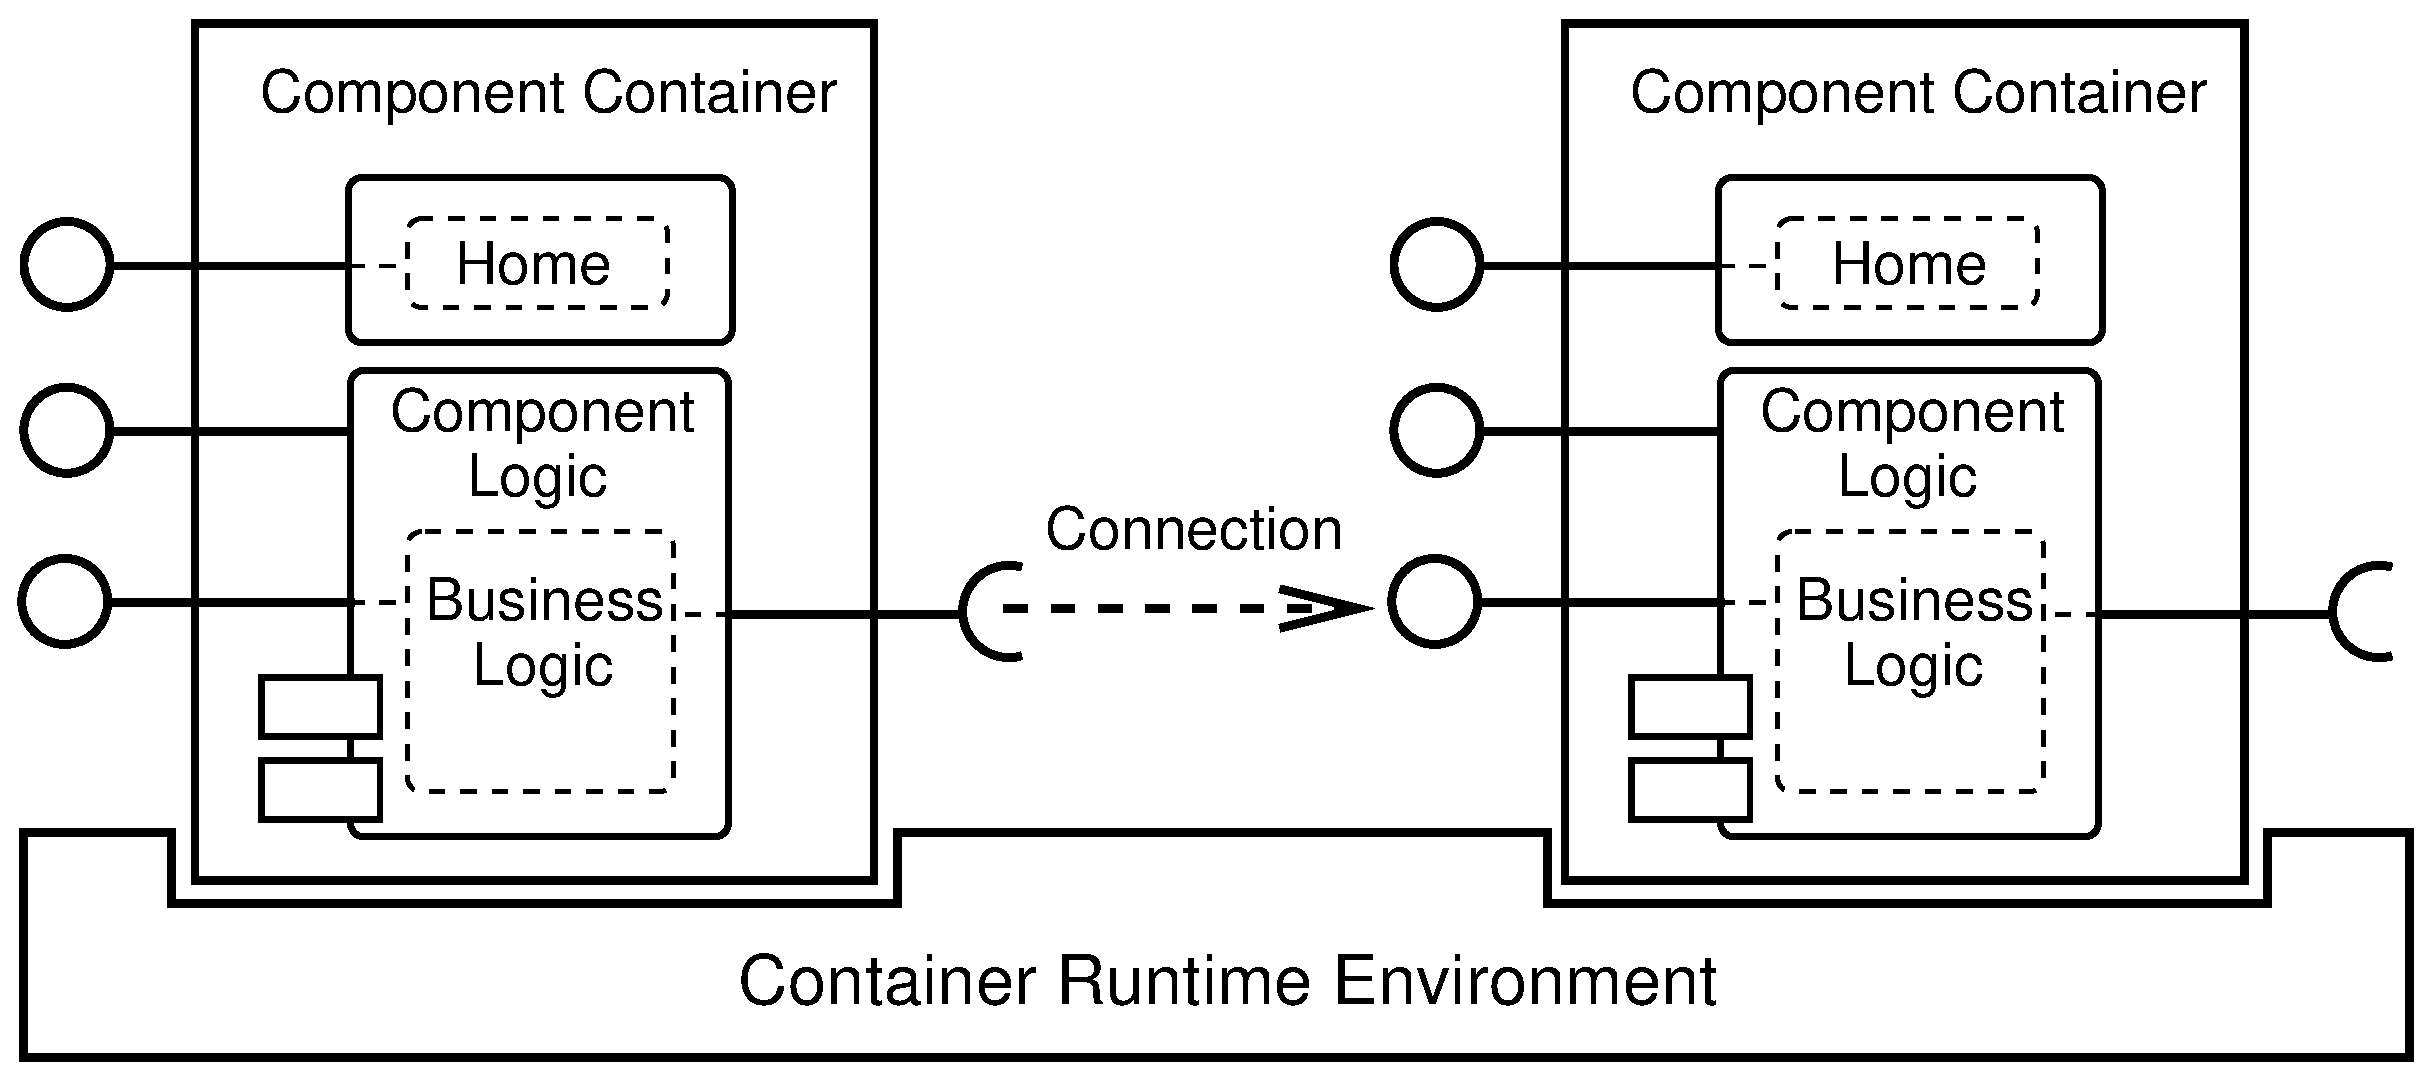
\includegraphics [width=10cm,angle=0] 
		     {figures/ContainerComponentlogicBusinesslogic.eps}
    \caption{A component implementation covers business logic, component
    logic, component container and container runtime environment.}
    \label{ContainerComponentlogicBusinesslogic}            
    \end{center}
\end{figure}

\begin{description}
\item [Business logic:]
  a component's business logic is written by the component developer to 
  implement   a domain specific functionality.
  Basically, business logic should not deal with technical aspects like contract
  verification or middleware API.
  
\item [Component logic:]
  business logic is embedded in a layer of generated code called component 
  logic. The interaction between business logic and component logic is well 
  defined in terms of interfaces (context interface, callback interface).
  Component logic handles technical aspects as well as a component's life-cycle.
  Additionally, component logic is glue code that fits a component into a 
  generic component container.
  
\item [Component container:]
  a component type is hosted by a component container that manages instances of
  that component type.
  While component logic is generated for each particular component type, the 
  component container is a generic part of the component platform.
  
\item [Container runtime environment:]
  a component platform also supports a set of libraries and services that can 
  be used by component containers.
  Any middleware used here is also part of this runtime environment.
\end{description}


\noindent
From this implementation schema, two different component views can be deduced:
\begin{description}
\item [External view:]
  a component provides its ports defined by interfaces. All 
  client calls to these ports are routed through the component container and 
  the generated component logic before business logic functionality is
  executed.
  
\item [Internal view:]
  a component's business logic can call methods on a context 
  object, which is part of generated component logic, and has to implement 
  a callback interface that allows the component container to handle the 
  component's life--cycle.
\end{description}


\noindent
Conforming with the concept of component model and 
middleware separation, we have implemented a local version of LwCCM components.
These local components host business logic and are completely independent 
from a particular middleware technology.

\begin{figure}[htbp]
    \begin{center}
    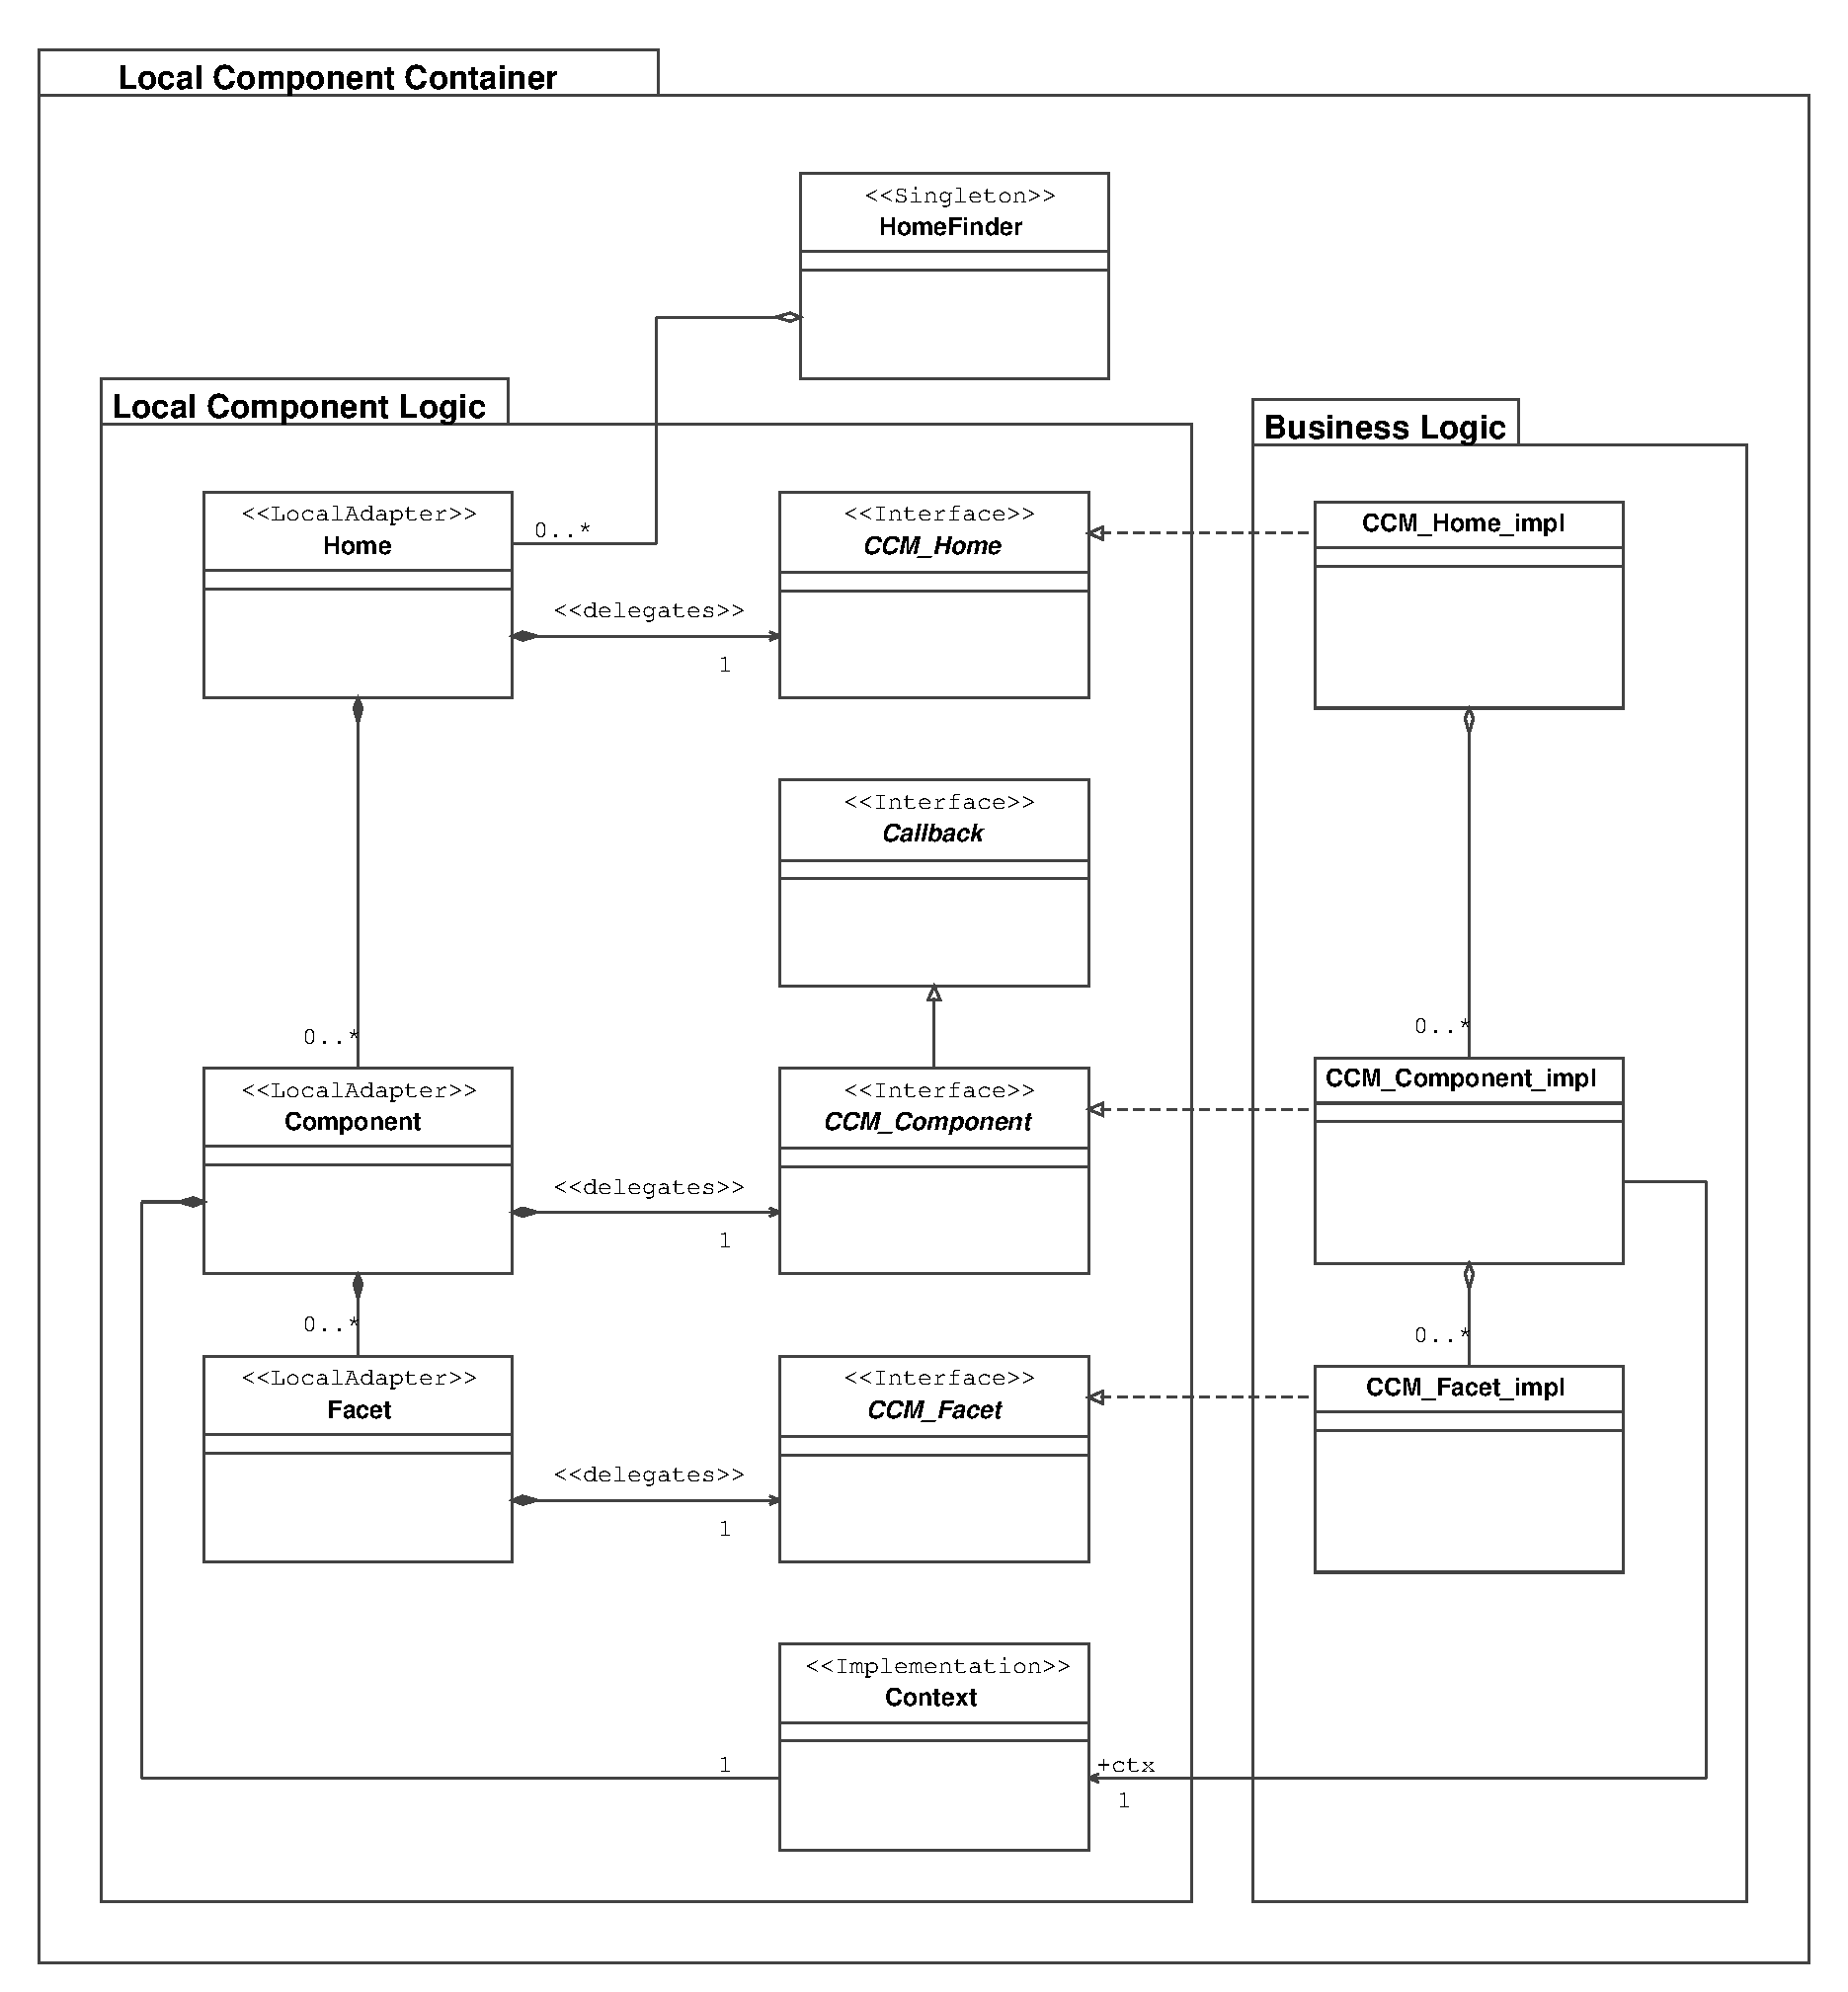
\includegraphics [width=15cm,angle=0] {uml/StructureOfLocalComponents.eps}
    \caption{This simplified structure of a local component implementation
    shows the relationship between business logic, local component logic and
    a local component container.}
    \label{StructureOfLocalComponents}            
    \end{center}
\end{figure}

\noindent
Implementations without middleware are much leaner and allow
finer grained components which are simpler to reuse.
Especially in languages that do not provide a native component model
(like C++), a local version of LwCCM can be useful.  

\newpage
\noindent
Based on this simplified class diagram, we can analyze the following
interactions between business logic and component logic:

\begin{description}
\item [Calling component methods:]
usually, a component client calls methods on a component's interface.
These interfaces can be either a component home, a component equivalent 
interface or a facet.
Invocations on all these interfaces follow the same structural pattern,
as shown in Fig.~\ref{LocalComponentImplementationStructure}.
A component's client calls methods on generated adapter classes 
that implements a component's interfaces. 
These adapters delegate calls 
to generated interfaces which are implemented by business logic classes.
\begin{figure}[htbp]
    \begin{center}
    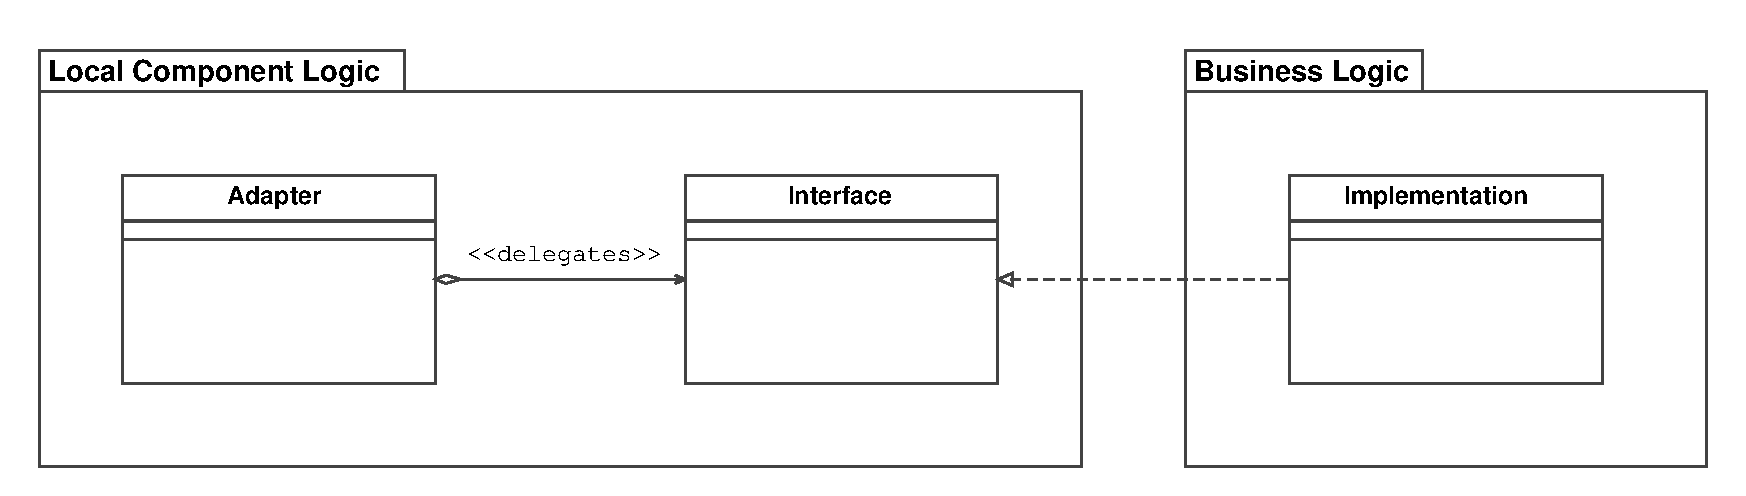
\includegraphics [width=13cm,angle=0] 
		     {uml/LocalComponentImplementationStructure.eps}
    \caption{Structure of a local component.}
    \label{LocalComponentImplementationStructure}            
    \end{center}
\end{figure}

This pattern implies two benefits:
\begin{itemize}
\item The adapter layer brings in an indirection that can be used to execute
some pre- and post-invocation functionality.  

\item Business logic can implement a well defined interface which is generated 
from the component model.
\end{itemize}

\item [Invoking callback methods:]
as shown in Fig.~\ref{StructureOfLocalComponents}, a generated component 
interface inherits the {\tt Callback} interface that defines methods which 
will be used by the component logic to control the business logic life-cycle.

\item [Using context methods:]
while calls from component clients as well as calls from component logic to 
the callback interface 
are directed from outside to the business logic, there is also
a need for interaction between business logic and generated glue code.

In the other direction, from business logic to component logic, a {\tt Context}
object is used to provide access to container functionality.
Additionally, business logic gets receptacle references from this context 
object, that are used to call methods defined by these receptacle interfaces.
Remember, receptacles are connected to facets which implement these common
interfaces.
\end{description}

\noindent
An important part of a local component container is the {\tt HomeFinder} class. 
This class is implemented as a singleton
\cite{Gamma95} and manages component home instances.
When a local LwCCM component is deployed, an instance of the component's home
is created and registered by the {\tt HomeFinder} using a unique name. 
After that, the {\tt HomeFinder} can be used to retrieve home references by 
their name.

\newpage
% $Id$
%==============================================================================
\section{Test--Driven Component Development}
\label{TestDrivenComponentDevelopment}
%==============================================================================

As we have seen from the Hello World example, components can be implemented in
a parallel task.
While system design describes the structure and interactions between 
components, component implementation constitutes the components behavior.

%------------------------------------------------------------------------------
\subsection{Component development process}
%------------------------------------------------------------------------------
The component development process defines activities needed to 
implement a component's business logic embedded in a generated 
component logic in a test--driven approach. 
Fig.~\ref{ProcessComponentDevelopment} shows the {\it write the test first}
paradigm used in test--driven component development.

\begin{figure}[htbp]
    \begin{center}
    \includegraphics [width=4.5cm,angle=0] {figures/ProcessComponentDevelopment.eps}
    \caption{A test--driven component development process.}
    \label{ProcessComponentDevelopment}            
    \end{center}
\end{figure}

\noindent
Two nested iteration cycles are shown in the diagram 
(Fig.~\ref{ProcessComponentDevelopment}). 
The inner iteration cycle 
is concerned with implementing and testing business logic to pass a particular 
test case.
The outer iteration cycle is started with every new test case derived from a 
functional requirement analysis.

\newpage
\noindent
The presented component development process contains the following activities: 
\begin{itemize}
\item {\bf Generate component.}
Based on component descriptions, tools can be used to 
generate platform specific component logic which can host the implemented 
business logic.

\item {\bf Analyze requirements.}
A component has to satisfy a set of functional requirements. The description 
of these requirements can be formally specified, modeled or written in prosa.

\item {\bf Implement test cases.}
From the requirements specifications, test cases can be implemented. 
These test cases express a component's usage in a particular programming 
language.
There will be a test case for every postulated aspect of the component's 
functionality.
Each executable test case augments the set of automated tests that can be
run again later for regression testing too.

\item {\bf Implement business logic.}
The business logic must be implemented in a way that the implemented test cases
can run without a failure. 
There is no need for a component developer to know the overall goal of the 
software system. 
The business logic is only determined by requirements expressed by executable
test cases.

\item {\bf Run test case.}
At every time in development, the business logic of a component can be checked
by running all implemented test cases.
Thus, there is a well defined end to component development - as soon as all 
test cases, that represents the functional requirements, are
running, the work is done.
\end{itemize}

\noindent
The fact, that each implementation of a component's functionality starts by 
writing a test case, automatically leads to testable business logic.
Another benefit of executable test cases is that - after a change in 
business code - the whole test suite can be run to ensure the functional 
integrity of the component's implementation. 


%------------------------------------------------------------------------------
\subsubsection{Component development roles}
%------------------------------------------------------------------------------
The test--driven component development process defines two development roles 
which are usually performed by the same person:

\begin{itemize}
\item {\bf Test developer.}
A test developer analyzes the functional requirements for a component's 
business logic and implements test cases that can verify these requirements 
automatically.
 
\item {\bf Component developer.}
A component developer implements a component's business logic in respect to the
given test cases. His work is done, when all tests run through. 
\end{itemize}


\newpage
%------------------------------------------------------------------------------
\subsection{Car rental example}
%------------------------------------------------------------------------------

As a simple example, we define a car rental component that can handle customers
and miles. For each customer we can evaluate driven miles and costs incurred. 
We will store all created IDL files in a {\tt CarRental} directory
\footnote
{
You can find this example source code in the 
{\tt ccmtools/test/tutorial/CarRental} directory.}:
\begin{small}
\begin{verbatim}
        CarRental/
        |-- Exceptions.idl
        |-- Customer.idl
        |-- CustomerMaintenance.idl
        |-- CustomerBusiness.idl
        `-- CarRental.idl
\end{verbatim}
\end{small}

Keep in mind that IDL files contain no specification of what exact action will 
be performed.
The component developer bears the responsibility of filling in the functionality
after the component logic has been generated.

\begin{small}
\begin{verbatim}
#ifndef __EXCEPTIONS_IDL__
#define __EXCEPTIONS_IDL__

module BigBusiness {
  exception CreateCustomerException{};
  exception RemoveCustomerException{};
  exception NoCustomerException{};
}; // End of module BigBusiness
#endif
\end{verbatim}
\end{small}
This first code snippet shows the definition of three IDL exceptions.
In order to get a namespace, we envelop these definitions using a module called 
{\tt BigBusiness}. 
To prevent IDL files from multiple including, we define {\it include guards} 
within each source file.



 
\begin{small}
\begin{verbatim}
#ifndef __CUSTOMER_IDL__
#define __CUSTOMER_IDL__

module BigBusiness {
  struct Customer {
    long id;
    string first_name;
    string last_name;
    double mileage;
  };
  typedef sequence<Customer> CustomerList;
}; // End of module BigBusiness
#endif
\end{verbatim}
\end{small}

In {\tt Customer.idl}, we define a structure of basic data types and a sequence 
of this structure type.
Again, there is a {\tt BigBusiness} module and an include guard.

\begin{small}
\begin{verbatim}
#ifndef __CUSTOMER_MAINTENANCE_IDL__
#define __CUSTOMER_MAINTENANCE_IDL__

#include"Exceptions.idl"
#include"Customer.idl"

module BigBusiness {
  interface CustomerMaintenance
  {
    void createCustomer(in Customer person) 
      raises (CreateCustomerException);
    Customer retrieveCustomer(in long id)  
      raises (NoCustomerException);
    CustomerList retrieveAllCustomers()  
      raises (NoCustomerException);
    void updateCustomer(in Customer person)  
      raises (NoCustomerException);
    void deleteCustomer(in long id)  
      raises (RemoveCustomerException);
  };
}; // End of module BigBusiness
#endif
\end{verbatim}
\end{small}
Customers must be handled in a database like way. 
Thus, {\tt CustomerMaintenance.idl} contains a 
{\it Create, Retrieve, Update and Delete} (CRUD) interface. 
To pick a particular {\tt Customer}, we use a customer id that is realized by 
an IDL long type.
Methods can throw exceptions in the case of illegal customer ids, create or 
remove problems. 


\begin{small}
\begin{verbatim}
#ifndef __CUSTOMER_BUSINESS_IDL__
#define __CUSTOMER_BUSINESS_IDL__

#include "Exceptions.idl"

module BigBusiness {
  interface CustomerBusiness
  {
    attribute double dollars_per_mile;
    void addCustomerMiles(in long id, in double miles) 
      raises(NoCustomerException);
    void resetCustomerMiles(in long id) 
      raises(NoCustomerException);
    double getCustomerMiles(in long id) 
      raises(NoCustomerException);
    double getCustomerDollars(in long id) 
      raises(NoCustomerException);
  };
}; // End of module BigBusiness
#endif
\end{verbatim}
\end{small}

Beside the pure data manipulation, we also need an interface that defines a
business functionality.
{\tt CustomerBusiness.idl} defines an attribute and some methods that operate
on the given customer data. 
If a parameter represents a wrong customer id, the {\tt NoCustomerException}
will be thrown.

\begin{small}
\begin{verbatim}
#ifndef __CAR_RENTAL_IDL__
#define __CAR_RENTAL_IDL__

#include "CustomerMaintenance.idl"
#include "CustomerBusiness.idl"

module BigBusiness {

  component CarRental 
  { 
    provides CustomerMaintenance maintenance;
    provides CustomerBusiness business;
  };
  
  home CarRentalHome manages CarRental 
  { };

}; // End of module BigBusiness
#endif
\end{verbatim}
\end{small}

Finally, we collect the included interfaces to a {\tt CarRental} component and 
define a {\tt CarRentalHome} that will be used to create component instances at
runtime.

Well done! We have defined our component in terms of IDL.


\vspace{10mm}
%------------------------------------------------------------------------------
\subsubsection{Generate component}
%------------------------------------------------------------------------------

In this step, we bring the IDL3 files in a proper structure that implies 
the separation between interface and component definitions. 
\begin{small}
\begin{verbatim}
> ccmtools idl3 -o server/idl3 *.idl
\end{verbatim}
\end{small}
A result of this CCM Tools call is the following file structure.
The separation between interface and component related files reflects the
fact that interfaces are used to defined components but are not owned by
these components.
\begin{small}
\begin{verbatim}
server
`-- idl3
    |-- component
    |   `-- BigBusiness
    |       |-- CarRental.idl
    |       `-- CarRentalHome.idl
    `-- interface
        `-- BigBusiness
            |-- CreateCustomerException.idl
            |-- Customer.idl
            |-- CustomerBusiness.idl
            |-- CustomerList.idl
            |-- CustomerMaintenance.idl
            |-- NoCustomerException.idl
            `-- RemoveCustomerException.idl
\end{verbatim}
\end{small}


To generate C++ source code from IDL3 we have to call the CCM Tools generator
twice, once for the interfaces and once for the component:
\begin{small}
\begin{verbatim}
> ccmtools c++local -o server/interface \
                    -Iserver/idl3/interface \
                     server/idl3/interface/BigBusiness/*.idl
> ccmtools c++local -a -o server/component/CarRental \
                    -Iserver/idl3/component \
                    -Iserver/idl3/interface \
                     server/idl3/component/BigBusiness/CarRental*.idl 
\end{verbatim}
\end{small}

Now, the {\tt server} directory contains the component's source code. 
(To get a description of all {\tt ccmtools} options consult the 
CCM Tools commands section in the tutorial's appendix).
\begin{small}
\begin{verbatim}
server
|-- idl3
|-- component
|   `-- CarRental
|       |-- CCM_Local_BigBusiness_CCM_Session_CarRental
|       |-- CCM_Local_BigBusiness_CCM_Session_CarRental_share
|       `-- impl
|           |-- CarRentalHome_entry.h
|           |-- CarRentalHome_impl.cc
|           |-- CarRentalHome_impl.h
|           |-- CarRental_business_impl.cc
|           |-- CarRental_business_impl.h
|           |-- CarRental_impl.cc
|           |-- CarRental_impl.h
|           |-- CarRental_maintenance_impl.cc
|           |-- CarRental_maintenance_impl.h
|           `-- Makefile.py
`-- interface
    `-- CCM_Local_BigBusiness
        |   |-- CreateCustomerException.h
        |   |-- Customer.h
        |   |-- CustomerBusiness.h
        |   |-- CustomerList.h
        |   |-- CustomerMaintenance.h
        |   |-- Makefile.py
        |   |-- NoCustomerException.h
        |   `-- RemoveCustomerException.h
        `-- Makefile.py
\end{verbatim}
\end{small}

The component developer really ought not to care about the generated 
{\tt CCM\_Local\_*} subdirectories (if you don't believe us, though, feel free 
to read through it; just don't edit anything). 
The interesting files are listed in the {\tt impl} directory. 
These files contain skeleton code (that are empty methods) of the component's 
business logic.

\begin{itemize}
\item {\tt CarRentalHome\_entry.h} \\
This file is the business logic's entry point and declares an extern ``C'' 
function that returns a component home instance.
The generated implementation of this function is hosted in the 
{\tt CarRentalHome\_impl.cc} file.

\item {\tt CarRentalHome\_impl.[h,cc]} \\
These files contain the factory methods for component instantiation. 
While user defined factory methods must be implemented manually, the default 
{\tt create} method is already generated.

\item {\tt CarRental\_impl.[h,cc]} \\
These files contain the implementation of supported interfaces as well as the
implementation of component attributes.

\item {\tt CarRental\_business\_impl.[h,cc]} \\
{\tt CarRental\_maintenance\_impl.[h,cc]} \\
These files contain the implementation of defined facets and builds
the component's business logic
(grep for {\tt // TODO : IMPLEMENT ME HERE !}).

\item {\tt Makefile.py} \\
This file is a Confix marker that denotes a directory as 'to compile'.
\end{itemize}

Files in the {\tt impl} directory are protected from overwriting.
Running the generator again results in a bunch of warnings. 
Instead of overwriting, the generator stores the new files with an extension 
({\tt *.new}) into the same directory.
You can make a {\tt diff} to figure out changes. 

\vspace{3mm}
The generated business logic skeletons contains enough code to be compilable.
Confix, our build tool, needs some informations about the package to build.
The following content must be placed in the {\tt server/Makefile.py} file:
\begin{small}
\begin{verbatim}
# server/Makefile.py
PACKAGE_NAME('CarRental')
PACKAGE_VERSION('1.0.0')
\end{verbatim}
\end{small}
Additionally, some empty {\tt Makefile.py} files must be placed in
source directories to force {\tt Confix} to build them:
\begin{small}
\begin{verbatim}
> touch server/interface/Makefile.py
> touch server/component/Makefile.py
> touch server/component/CarRental/Makefile.py
\end{verbatim}
\end{small}

Finally, to build the generated {\tt Carrental} component, type:
\begin{small}
\begin{verbatim}
> confix.py --packageroot=`pwd`/server --bootstrap --configure --make
\end{verbatim}
\end{small}



%------------------------------------------------------------------------------
\subsubsection{Mirror Component Concept (MCC)}
%------------------------------------------------------------------------------

Software development is an iterative process. Kent Beck
has proposed a {\it Test Driven Development} (TDD) methodology 
\cite{Beck2003TDD} that starts by
implementing the test~-- before implementing the business logic!

As shown in Fig.~\ref{fig:test-driven-development}, the CCM Tools make use of
the TDD idea in the context of components. For every component $C$, we
generate a mirror component $\overline{C}$. Each input port (receptacle)
of $C$ corresponds to an output port (facet) of $\overline{C}$, and vice versa.

\begin{figure}[htb]
    \begin{center}
    \includegraphics [width=5cm,angle=0] {figures/TestArchitecture.eps}
    \caption{A Component test architecture consists of a 
      $(C, \overline{C})$ pair that is managed by a test client.}
    \label{fig:test-driven-development}
    \end{center}
\end{figure}

Fig.~\ref{TestClientSequenceDiagramm} shows the sequence diagram for this 
automatic test concept.
Basically, a mirror component test is made up of three execution phases:

\begin{itemize}
\item Setup phase (step 1 to 10): \\
Before a test case can be executed, the mirror component test environment must
be established.
First, both components must be created and configured by their attributes.
$C$ and $C\_mirror$ hold the same attribute set,
thus, both components can be configured in the same way. 
Then, $C$ and $C\_mirror$ are connected with each other.

Calling {\tt configuration\_complete} finishes this build--up phase.

\item Testing phase (step 11):\\
In this phase all test cases implemented in $C\_mirror$ are executed.
Remember, after a {\tt configuration\_complete} call from a client, the 
container calls a component's {\tt ccm\_activate} callback method.
Test cases can be implemented in or called from this callback
method. 
As all test cases are implemented within a component, a test 
developer can use the same programming paradigm as a component developer. 

\item Tear down phase (step 12 to 15): \\
After all test cases have finished, the mirror component test environment must 
be destroyed.
All connections between $C$ and $C\_mirror$ must be disconnected and both
components must be removed. 
\end{itemize}

\begin{figure}[htb]
    \begin{center}
      \includegraphics [width=9.5cm,angle=0] 
		       {figures/TestClientSequenceDiagram.eps}
    \caption{Automatic test procedure based on the mirror component 
      test concept.}
    \label{TestClientSequenceDiagramm}            
    \end{center}
\end{figure}

\noindent
A component test spans from component creation to component destruction.
Thus, we have implemented a full component life cycle test environment that
is the assumption to implement components in a test driven way.

Because a mirror component can be used as an executable semantic description of 
a component's business logic, component development can stop as soon as all 
mirror component test cases run through. 

To create a mirror component $\overline{C}$ definition from existing
IDL3 files, type:
\begin{small}
\begin{verbatim}
> ccmtools idl3mirror -o server/idl3 \
                      -Iserver/idl3/interface \
                      -Iserver/idl3/component \
                      server/idl3/component/BigBusiness/CarRental*.idl
\end{verbatim}
\end{small}

From the generated IDL3 files you can see that both $\overline{C}$ and $C$ 
uses the same interfaces.
\begin{small}
\begin{verbatim}
server
`-- idl3
    |-- component
    |   `-- BigBusiness
    |       |-- CarRental.idl
    |       |-- CarRentalHome.idl
    |       |-- CarRentalHome_mirror.idl    // new
    |       `-- CarRental_mirror.idl        // new
    `-- interface
        `-- BigBusiness
            |-- CreateCustomerException.idl
            |-- Customer.idl
            |-- CustomerBusiness.idl
            |-- CustomerList.idl
            |-- CustomerMaintenance.idl
            |-- NoCustomerException.idl
            `-- RemoveCustomerException.idl
\end{verbatim}
\end{small}

Now we can use the regular {\tt c++local} generator to create C++ component 
logic from the IDL3 mirror files.
\begin{small}
\begin{verbatim}
> ccmtools c++local -a -o server/component/CarRental_mirror \
                       -Iserver/idl3/interface \
                       -Iserver/idl3/component \
                       server/idl3/component/BigBusiness/CarRental*_mirror.idl
\end{verbatim}
\end{small}
This results in the following file structure:
\begin{small}
\begin{verbatim}
server
|-- component
|   |-- CarRental
|   `-- CarRental_mirror
|       |-- CCM_Local_BigBusiness_CCM_Session_CarRental_mirror
|       |-- CCM_Local_BigBusiness_CCM_Session_CarRental_mirror_share
|       `-- impl
|           |-- CarRentalHome_mirror_entry.h
|           |-- CarRentalHome_mirror_impl.cc
|           |-- CarRentalHome_mirror_impl.h
|           |-- CarRental_mirror_impl.cc
|           |-- CarRental_mirror_impl.h
|           `-- Makefile.py
\end{verbatim}
\end{small}

The {\tt impl} directory contains generated files of the mirror
component's business logic that can host component test cases.
In the next sections of this tutorial, we will implement test cases as well
as business logic. 


Finally, a test client that coordinates creation and connecting of 
component $C$ and mirror component $\overline{C}$ must be added.
To generate this test client, we type:
\begin{small}
\begin{verbatim}
> ccmtools c++local-test -o server/component/CarRental_mirror \
                         -Iserver/idl3/interface \
                         -Iserver/idl3/component \
                         server/idl3/component/BigBusiness/CarRental.idl
\end{verbatim}
\end{small}

The generated files are stored in the following way:
\begin{small}
\begin{verbatim}
server
|-- component
|   |-- CarRental
|   `-- CarRental_mirror
|       |-- CCM_Local_BigBusiness_CCM_Session_CarRental_mirror
|       |-- CCM_Local_BigBusiness_CCM_Session_CarRental_mirror_share
|       |-- impl
|       `-- test
|           |-- Makefile.py
|           `-- _check_CCM_Local_BigBusiness_CCM_Session_CarRental.cc
\end{verbatim}
\end{small}

The {\tt test} directory contains a generated {\tt \_check\_*} file that 
contains the test client and is also protected from overwriting.

Before we can use {\tt Confix} to build the mirror component and run the
test case, a {\tt Makefile.py} file must sign the new component directory:
\begin{small}
\begin{verbatim}
> touch server/component/CarRental_mirror/Makefile.py

> confix.py --packageroot=`pwd`/server --bootstrap --configure 
            --make --targets=check 
\end{verbatim}
\end{small}


\newpage
%------------------------------------------------------------------------------
\subsubsection{Implement test cases}
%------------------------------------------------------------------------------

Now is a good time to start the development of business code. First, we have to
define the behavior of the business code in an executable semantic. 
In other words, we write a test case in the mirror component 
({\tt CarRental\_mirror\_impl.cc}):

\begin{small}
\begin{verbatim}
void CCM_CarRental_mirror_impl::ccm_activate()
    throw (LocalComponents::CCMException)
{
    try {
      {
          CCM_Local::BigBusiness::Customer person;
          person.id = 1;
          person.first_name = "Franz";
          person.last_name = "Kafka";
          ctx->get_connection_maintenance_mirror()->
              createCustomer(person);
      }
      {
          CCM_Local::BigBusiness::Customer person;
          long id = 1;
          person = ctx->get_connection_maintenance_mirror()->
              retrieveCustomer(id);
          assert(person.id == 1);
          assert(person.first_name == "Franz");
          assert(person.last_name == "Kafka");
      }
  }
  catch(CCM_Local::BigBusiness::CreateCustomerException) {
      cerr << "MAINTENANCE ERROR: Can't create customer!" << endl;
  }
  catch(CCM_Local::BigBusiness::NoCustomerException) {
      cerr << "MAINTENANCE ERROR: no customer found!" << endl;
  }
}
\end{verbatim}
\end{small}
The test case is implemented in the {\tt ccm\_activate()} callback method of the
mirror component because this method is called after creating and connecting $C$
and $\overline{C}$ from the component logic. 

First, we create a valid {\tt Customer} record and  
use the context object ({\tt ctx}) to get a smart pointer
to $\overline{C}$'s receptacle (which is connected with $C$'s facet) 
before we call the {\tt createCustomer} operation. 
After that, we retrieve the record from the receptacle and compare the stored 
items.

To compile and run the test, we call {\tt Confix} as before:
\begin{small}
\begin{verbatim}
> confix.py --packageroot=`pwd`/server --bootstrap --configure 
            --make --targets=check 
\end{verbatim}
\end{small}
The test failed! 
That's fine because there is no business code to work with...






%------------------------------------------------------------------------------
\subsubsection{Implement business logic}
%------------------------------------------------------------------------------

Now we are ready to implement the business logic that satisfies the written 
test case. 
First, we implement the customer database - no panic - we 
simple put a C++ {\tt std::vector<>} into the {\tt CarRental\_impl.h} file,
to hold {\tt Customer} entities.

\begin{small}
\begin{verbatim}
class CCM_CarRental_impl : virtual public CCM_CarRental
{
  public:
    std::vector<CCM_Local::BigBusiness::Customer> CustomerDB;
    //...
};
\end{verbatim}
\end{small}

Next, we open {\tt CarRental\_maintenance\_impl.cc} and add the following 
lines:
\begin{small}
\begin{verbatim}
void
maintenance_impl::createCustomer ( const Customer& person )
  throw (LocalComponents::CCMException, CreateCustomerException)
{
  component->CustomerDB.push_back(person);
}

Customer
maintenance_impl::retrieveCustomer ( const long id )
  throw (LocalComponents::CCMException, NoCustomerException)
{
  std::vector<CCM_Local::BigBusiness::Customer>::iterator pos;
  for(pos = component->CustomerDB.begin(); 
      pos != component->CustomerDB.end(); ++pos) {
    if(pos->id == id) {
      return *pos;
    }
  }
  throw NoCustomerException();
}
\end{verbatim}
\end{small}

Instead of a database, we simply use a {\tt std::vector<>} to implement
the {\tt createCustomer} and {\tt retrieveCustomer} methods - that's it! 

We'll run the test again to see if it's working:
\begin{small}
\begin{verbatim}
> confix.py --packageroot=`pwd`/server --make --targets=check
\end{verbatim}
\end{small}

Yay, the test passed!



%------------------------------------------------------------------------------
\subsubsection{Implement test case, implement business logic, run test case...}
%------------------------------------------------------------------------------

The idea of test driven development is to run short cycles of test and
implementation until all required functionality is implemented.
For the {\tt CarRental} component, this section goes through all these 
development steps. 
To keep the tutorial clean, we implement only simple tests that show the
functionality of {\tt CarRental}'s business logic.
In practice, these white box tests must be much more substantial.

\begin{small}
\begin{verbatim}
    {
      CCM_Local::BigBusiness::Customer person;

      person.id = 2;
      person.first_name = "Thomas";
      person.last_name = "Bernhard";
      ctx->get_connection_maintenance_mirror()->
           createCustomer(person);

      person.id = 3;
      person.first_name = "Karl";
      person.last_name = "Kraus";
      ctx->get_connection_maintenance_mirror()->
           createCustomer(person);
    }
\end{verbatim}
\end{small}

To test the {\tt retrieveAllCustomers} method, we add two other customers before
we call the method. All retrieved records are compared with their initial values
to validate the query results. 

\begin{small}
\begin{verbatim}
    {
      CCM_Local::BigBusiness::CustomerList person_list;

      person_list = ctx->get_connection_maintenance_mirror()->
                         retrieveAllCustomers();
      assert(person_list.at(2).id == 3);
      assert(person_list.at(2).first_name == "Karl");
      assert(person_list.at(2).last_name == "Kraus");

      assert(person_list.at(1).id == 2);
      assert(person_list.at(1).first_name == "Thomas");
      assert(person_list.at(1).last_name == "Bernhard");

      assert(person_list.at(0).id == 1);
      assert(person_list.at(0).first_name == "Franz");
      assert(person_list.at(0).last_name == "Kafka");
    }      
\end{verbatim}
\end{small}

The method's implementation creates a new {\tt CustomerList} which
is returned by value.
In the case of an empty list the {\tt NoCustomerException} is thrown.

\begin{small}
\begin{verbatim}
CustomerList maintenance_impl::retrieveAllCustomers (  )
  throw (LocalComponents::CCMException, NoCustomerException )
{
  if(component->CustomerDB.size() == 0)
      throw NoCustomerException();
  CCM_Local::BigBusiness::CustomerList customer_list;
  std::vector<CCM_Local::BigBusiness::Customer>::iterator pos;
  for(pos = component->CustomerDB.begin(); 
      pos != component->CustomerDB.end(); ++pos) {
    customer_list.push_back(*pos);
  }
  return customer_list;
}
\end{verbatim}
\end{small}

Next, we implement a test case for {\tt updateCustomer}.
A new {\tt Customer} record is created and used as parameter.
To check the update procedure, we use {\tt retrieveCustomer} 
and compare the result record with the new values.

\begin{small}
\begin{verbatim}
    {
      CCM_Local::BigBusiness::Customer person;
      person.id = 1;
      person.first_name = "Werner";
      person.last_name = "Schwab";
      double mileage = 0.0;
      ctx->get_connection_maintenance_mirror()->
           updateCustomer(person);      

      CCM_Local::BigBusiness::Customer another_person;
      another_person = 
        ctx->get_connection_maintenance_mirror()->
             retrieveCustomer(person.id);
      assert(another_person.id == 1);
      assert(another_person.first_name == "Werner");
      assert(another_person.last_name == "Schwab");
    }
\end{verbatim}
\end{small}



To implement {\tt updateCustomers} we simply iterate through the {\tt Customer}
vector and compare each item with the given person.
If person matches, we overwrite the vector item and return.
If person does not match, {\tt NoCustomerException} is thrown.

\begin{small}
\begin{verbatim}
void maintenance_impl::updateCustomer ( const Customer& person )
  throw (LocalComponents::CCMException, NoCustomerException )
{
  std::vector<CCM_Local::BigBusiness::Customer>::iterator pos;
  for(pos = component->CustomerDB.begin(); 
      pos != component->CustomerDB.end(); ++pos) {
    if(pos->id == person.id) {
      *pos = person;
      return;
    }
  }
  throw NoCustomerException();  
}
\end{verbatim}
\end{small}


In the following test case, we delete a {\tt Customer} and try to retrieve the 
deleted record.
If this works, we break the test ({\tt assert(false)}) because this would be an
incorrect behavior. 
Instead, the {\tt RemoveCustomerException} must be thrown.
\begin{small}
\begin{verbatim}
    {
      long id = 1;
      ctx->get_connection_maintenance_mirror()->
           deleteCustomer(id);
      CCM_Local::BigBusiness::Customer person;
      person = ctx->get_connection_maintenance_mirror()->
                    retrieveCustomer(id);
      assert(false); // Customer found => error
    }
\end{verbatim}
\end{small}

\begin{small}
\begin{verbatim}
void maintenance_impl::deleteCustomer ( const long id )
  throw (LocalComponents::CCMException, RemoveCustomerException)
{
  std::vector<CCM_Local::BigBusiness::Customer>::iterator pos;
  for(pos = component->CustomerDB.begin(); 
      pos != component->CustomerDB.end(); ++pos) {
    if(pos->id == id) {
      component->CustomerDB.erase(pos);
      return;
    }
  }
  throw RemoveCustomerException();  
}
\end{verbatim}
\end{small}

We iterate through the {\tt Customer} vector and compare 
each item with the given id.
If the given record is found, we will remove it from the {\tt Customer} vector.
If the given id can't be found in the{\tt Customer} vector, 
{\tt RemoveCustomerException} is thrown.
In conclusion, we have implemented the whole {\tt maintenance} facet hand in 
hand with its test cases. 

\vspace{3mm}
A great benefit of test driven development is that testing is not longer a 
separated part at the end of a software development process.
In practice, most projects are running out of time before testing can start. 
Thus, lots of functionality is implemented but test cases are skipped 
frequently.
With a test driven approach, one can scale the functionality of a project when 
time is running out, but ensure software quality by having automatic tests.

Another benefit of automatic tests appear in context of code refactoring. 
After making some changes in a component's implementation, we can run all test 
cases to ensure that its functionality is still available.


In order to implement the second facet, we start with a new test case in 
$\overline{C}$.
For {\tt business} facet tests, we create a new try/catch block that catches
only {\tt NoCustomerException}s.
 
The test adds some miles to an existing customer, retrieves the current miles 
value from the same customer and verifies their equality. 

\begin{small}
\begin{verbatim}
  try {
    {
      long id = 2;
      double miles = 197.7;

      ctx->get_connection_business_mirror()->
           addCustomerMiles(id, miles); 

      double other_miles;
      other_miles = 
        ctx->get_connection_business_mirror()->
             getCustomerMiles(id); 
      assert( abs(other_miles - miles) < 0.001);
    }
  }
  catch(CCM_Local::BigBusiness::NoCustomerException) {
    cerr << "MAINTENANCE ERROR: no customer found!" << endl;
    assert(false);
  }
\end{verbatim}
\end{small}


To make the test run, we have to implement two facet methods.
{\tt addCustomerMiles} iterates through the {\tt Customer} vector
and compares the id values.
If the given {\tt Customer} id is found, the miles value is added to
its current status.
If the given id does not match, a {\tt NoCustomerException} is thrown.
\begin{small}
\begin{verbatim}
void business_impl::addCustomerMiles(const long id, 
                                     const double miles)
  throw (LocalComponents::CCMException, NoCustomerException )
{
  std::vector<CCM_Local::BigBusiness::Customer>::iterator pos;

  for(pos = component->CustomerDB.begin(); 
      pos != component->CustomerDB.end(); ++pos) {
    if(pos->id == id) {
      pos->mileage += miles;
      return;
    }
  }
  throw NoCustomerException();    
}
\end{verbatim}
\end{small}

After adding miles to an existing {\tt Customer} we have to implement a method
that get the current value of a {\tt Customer}'s mileage member.

\begin{small}
\begin{verbatim}
double business_impl::getCustomerMiles ( const long id )
  throw (LocalComponents::CCMException, NoCustomerException )
{
  std::vector<CCM_Local::BigBusiness::Customer>::iterator pos;

  for(pos = component->CustomerDB.begin(); 
      pos != component->CustomerDB.end(); ++pos) {
    if(pos->id == id) {
      return pos->mileage;
    }
  }
  throw NoCustomerException(); 
}
\end{verbatim}
\end{small}

Again, we iterate through the {\tt Customer} vector and compare the id values.
If we find a {\tt Customer} with the right id, we read its mileage value and
return it to the caller.
In the other case, as usual, the {\tt NoCustomerException} is thrown.


The following test case sets the facet's {\tt dollars\_per\_mile} attribute
and retrieves the current mileage and Dollar status of a particular 
{\tt Customer} determined by its id.
Thus, the component's calculation can be verified.

\begin{small}
\begin{verbatim}
    {
      long id = 2;
      double dollars, miles;
      double factor = 5.3;
      ctx->get_connection_business_mirror()->
           dollars_per_mile(factor);
      miles = ctx->get_connection_business_mirror()->
                   getCustomerMiles(id);
      dollars = ctx->get_connection_business_mirror()->
                     getCustomerDollars(id); 
      assert( abs(dollars - miles*factor) < 0.001);
    }
\end{verbatim}
\end{small}

Note that a standard implementation of a facet's attribute will be
generated by CCM Tools.

The following code implements the {\tt getCustomerDollars()} method:
\begin{small}
\begin{verbatim}
double business_impl::getCustomerDollars ( const long id )
  throw (LocalComponents::CCMException, NoCustomerException )
{
  return getCustomerMiles(id) * _dollars_per_mile;
}
\end{verbatim}
\end{small}

Life would be pretty ease if all business logic would be as simple to implement 
as this method ;-)


\newpage
Finally, the last test case resets a {\tt Customer}'s mileage value and 
retrieves its Dollar status. Of course, it has to be null.

\begin{small}
\begin{verbatim}
    {
      long id = 2;
      double dollars;
      ctx->get_connection_business_mirror()->
           resetCustomerMiles(id);
      dollars = 
        ctx->get_connection_business_mirror()->
             getCustomerDollars(id); 
      assert( abs(dollars) < 0.001);
    }
\end{verbatim}
\end{small}

{\tt resetCustomerMiles()} searches in the {\tt Customer}
vector for the given id and set the mileage value to null.
If no {\tt Customer} id matches, the {\tt NoCustomerException} is thrown.

\begin{small}
\begin{verbatim}
void business_impl::resetCustomerMiles ( const long id )
  throw (LocalComponents::CCMException, NoCustomerException )
{
  std::vector<CCM_Local::BigBusiness::Customer>::iterator pos;
  for(pos = component->CustomerDB.begin(); 
      pos != component->CustomerDB.end(); ++pos) {
    if(pos->id == id) {
      pos->mileage = 0.0;
      return;
    }
  }
  throw NoCustomerException(); 
}
\end{verbatim}
\end{small}

Well done! You have implemented the whole component in a test--driven
way using CCM Tools.



%------------------------------------------------------------------------------
\subsubsection{Install the {\tt CarRental} component}
%------------------------------------------------------------------------------

Installing a component means that the component's libraries and header files 
will be stored in a component repository, which is simply a directory on your 
computer (specified by {\tt PREFIX} in {\tt ~/.confix}).

Component installation is performed by Confix:
\begin{small}
\begin{verbatim}
> confix.py --packageroot=`pwd`/server/component \
            --make --targets=install
\end{verbatim}
\end{small}

\newpage
After installing a component, the component repository contains the following
file structures:
\begin{small}
\begin{verbatim}
include/
|-- CCM_Local
|   |-- BigBusiness
|   |   |-- CCM_Session_CarRental/
|   |   |-- CCM_Session_CarRental_mirror/
|   |   |-- CreateCustomerException.h
|   |   |-- Customer.h
|   |   |-- CustomerBusiness.h
|   |   |-- CustomerList.h
|   |   |-- CustomerMaintenance.h
|   |   |-- NoCustomerException.h
|   |   `-- RemoveCustomerException.h
\end{verbatim}
\end{small}

\begin{tiny}
\begin{verbatim}
lib/
|-- libCarRental_component_CarRental_CCM_Local_BigBusiness_CCM_Session_CarRental.a
|-- libCarRental_component_CarRental_impl.a
|-- libCarRental_component_CarRental_mirror_CCM_Local_BigBusiness_CCM_Session_CarRental_mirror.a
`-- libCarRental_component_CarRental_mirror_impl.a
\end{verbatim}
\end{tiny}


%------------------------------------------------------------------------------
\subsubsection{Implement a {\tt CarRental} client}
%------------------------------------------------------------------------------

A component based application builds up component assemblies using installed
components. In this section we will show this using a simple client that
instantiates the {\tt CarRental} component and calls the component's operations.

First, we add a {\tt client} directory to our project and implement
the client code in the {\tt src} subdirectory:
\begin{small}
\begin{verbatim}
CarRental/
|-- server/
`-- client
    |-- Makefile.py
    `-- CarRentalClient.cc
\end{verbatim}
\end{small}

Don't forget to implement the {\tt client/Makefile.py} file:
\begin{small}
\begin{verbatim}
PACKAGE_NAME('CarRentalClient')
PACKAGE_VERSION('1.0.0')
\end{verbatim}
\end{small}

First, a client needs a bunch of included header files that are generated by 
the CCM Tools.
There are different namespaces defined in the header files that we are using 
in the client code.

Second, the client's main function contains all the necessary code to use
the local {\tt CarRental} component. 
\begin{itemize}
\item Client's bootstrap and tear--down code.\\
Before a component can be used, a component home must be instantiated and 
registered by the {\tt HomeFinder}.
After using a component, the component home instance must be removed from 
memory and from the {\tt HomeFinder}'s list.
\item Component's instantiation code. \\
A client gets a home reference from the {\tt HomeFinder}, creates a component 
instance and asks for the component's facets.
To denote the end of this instantiation phase, the client calls 
{\tt configuration\_complete()}.
After all business calls, the client has to remove its component instance.

\item Client's application code. \\
Here the client calls some component operations to make its business work.
We have implemented a simple use case known from our mirror component test 
cases.
\end{itemize}

\begin{small}
\begin{verbatim}
#include <LocalComponents/CCM.h>
#include <CCM_Local/HomeFinder.h>
#include <WX/Utils/debug.h>
#include <WX/Utils/smartptr.h>

#include <CCM_Local/BigBusiness/CCM_Session_CarRental/CarRentalHome_gen.h>
#include <CCM_Local/BigBusiness/CCM_Session_CarRental/CarRental_gen.h>

using namespace std;
using namespace WX::Utils;
using namespace CCM_Local;
using namespace BigBusiness;
using namespace CCM_Session_CarRental;

int main(int argc, char *argv[])
{
  int error = 0;
  LocalComponents::HomeFinder* homeFinder;

  // Component deployment
  homeFinder = HomeFinder::Instance (  );
  error  = deploy_CCM_Local_BigBusiness_CarRentalHome("CarRentalHome");
  if(error) {
    cerr << "BOOTSTRAP ERROR: Can't deploy component homes!" << endl;
    return(error);
  }

  // Component instantiation
  try {
    SmartPtr<CarRentalHome> 
        myCarRentalHome(dynamic_cast<CarRentalHome*>
           (homeFinder->find_home_by_name("CarRentalHome").ptr()));

    SmartPtr<CarRental> myCarRental = myCarRentalHome->create();

    SmartPtr<CCM_Local::BigBusiness::CustomerMaintenance> 
      maintenance = myCarRental->provide_maintenance();    
    SmartPtr<CCM_Local::BigBusiness::CustomerBusiness> 
      business = myCarRental->provide_business();

    myCarRental->configuration_complete();

    // Use component
    CCM_Local::BigBusiness::Customer person;
    person.id = 1;
    person.first_name = "Franz";
    person.last_name = "Kafka";
    maintenance->createCustomer(person);

    business->addCustomerMiles(1, 120.0); 
    person = maintenance->retrieveCustomer(1);
    double dollars = business->getCustomerDollars(1); 

    cout << " Customer: " << person.first_name 
         << " " << person.last_name << endl;
    cout << " Miles: " <<  person.mileage << endl;
    cout << " to pay: " << dollars << " Dollars" << endl;

    // Destroy component instance
    myCarRental->remove();
  } 
  catch ( ... )  {
    cout << "Client: there is something wrong!" << endl;
    error = -1;
  }

  // Component tear down:
  error += undeploy_CCM_Local_BigBusiness_CarRentalHome("CarRentalHome");
  if(error) {
    return error;
  }
}
\end{verbatim}
\end{small}

To build and run the client application, we say:
\begin{small}
\begin{verbatim}
> confix.py --packageroot=`pwd`/client --bootstrap --configure 
            --make --target=install

> $CCM_INSTALL/bin/CarRentalClient_CarRentalClient
\end{verbatim}
\end{small}
% $ 

The advantage here is that development of local components is separated from
client development. 
While components can be implemented in independently by different developers, an
application (or client) can use deployed components from a repository.


\newpage
%------------------------------------------------------------------------------
\subsubsection{Uninstall the {\tt CarRental} client}
%------------------------------------------------------------------------------

To remove the client from the {\tt Confix} install repository, type:

\begin{small}
\begin{verbatim}
> confix.py --packageroot=`pwd`/client --make --target=uninstall
\end{verbatim}
\end{small}




%------------------------------------------------------------------------------
\subsubsection{Uninstall the {\tt CarRental} component}
%------------------------------------------------------------------------------

To remove the component from the {\tt Confix} install repository, type:

\begin{small}
\begin{verbatim}
> confix.py --packageroot=`pwd`/server --make --target=uninstall
\end{verbatim}
\end{small}

Installing is not necessary during component development. 
For implementing test cases and business logic we only need the source and
build directory (specified by {\tt BUILDROOT} in {\tt ~/.confix}).
 

\newpage
% $Id$
%==============================================================================
\chapter{Debugging Components}
%==============================================================================

CCM Tools generate additional debug informations within the local and
remote component adapters.

For each primitive type (e.g. long, string, etc.)
the {\tt cpp-environment} package contains {\tt ccmDebug()} 
functions that returns a string representation.
For user defined types, CCM Tools generate such {\tt ccmDebug()}
functions as part of the IDL to C++ mapping.   


%------------------------------------------------------------------------------
\section{WXDEBUG}
%------------------------------------------------------------------------------

As part of the {\tt wx-utils} package, a bunch of debug macros have been
defined. These macros can be used to write debug informations to the console
or another location.

To activate the wx-utils debug mechanism you have to define the {\tt WXDEBUG} 
macro, e.g. in the {\tt .confix} file:
\begin{verbatim} 
    'CONFIGURE': {
       'ENV': {
          'CC': 'gcc',
          'CXX': 'g++',      
          'CFLAGS': "-g -O0 -Wall -DWXDEBUG",
          'CXXFLAGS': "-g -O0 -Wall -DWXDEBUG",
       },
    }
\end{verbatim} 

After compiling generated components with {\tt -DWXDEBUG} you can activate
debug output via the {\tt WX\_DEBUG\_LEVELS} environment variable, e.g.:
\begin{verbatim} 
 > export WX_DEBUG_LEVELS="CCM_LOCAL CCM_REMOTE"
\end{verbatim} 

Currently, the following debug levels are supported by CCM Tools:
\begin{itemize}
\item {\tt CCM\_LOCAL} \\
Each method call to a local component's facet or supported interface
as well as attribute accesses will be recorded (including their C++ parameter
values and types).

\item {\tt CCM\_REMOTE} \\
Each method call to a CORBA component's facet or supported interface
as well as attribute accesses will be recorded (including their CORBA 
parameter values and types). Calls through receptacle adapters will not
be logged.

\item {\tt CCM\_CONTAINER} \\
Each method that is not directly related to a business call (e.g. constructors,
destructors or container management stuff) can be traced by activating this 
debug level.
\end{itemize}

You can also add your own debug levels to business logic. Simply add
wx-utils debug macros to your code as shown in the following code snippet:
\begin{verbatim}
  LDEBUGNL(LEVEL_1, "Message from debug level" << 1);
  LDEBUGNL(LEVEL_2, "Message from debug level" << 1+1);
  LDEBUGNL(LEVEL_3, "Message from debug level" << 1+1+1);
\end{verbatim}
Now, you can add {\tt LEVEL\_1}, {\tt LEVEL\_2} or {\tt LEVEL\_3} to the 
{\tt WX\_DEBUG\_LEVELS} environment variable to switch on and off debugging
messages.

Of course, there are much more features out there - have a look at the wx-utils
source code ;-)
\begin{verbatim}
wx-utils-1.2.0
|-- code
|   |-- CerrDebugWriter.cpp
|   |-- CerrDebugWriter.h
|   |-- CerrDebugWriter.o
|   |-- DebugWriter.h
|   |-- DebugWriterMgr.cpp
|   |-- DebugWriterMgr.h
|   |-- DebugWriterMgr.o
|   |-- debug.cc
|   |-- debug.h
\end{verbatim}
\newpage
% $Id$
%==============================================================================
\chapter{UML Component Design}
%==============================================================================

Remember, component based development starts with component design.
A component designer specifies components using the 
{\it Interface Definition Language} (IDL).

On the other side, the OMG proposes a {\it Model Driven Architecture} (MDA) 
where development starts at abstract levels called 
{\it Platform Independent Models} (PIM).
After some refinement steps, these PIM are transformed to 
{\it Platform Specific Models} (PSM).
Finally, from PSM, tools can generate source code that implements the modeled 
application.

OK, that's the vision. 
In practice, there are still problems in applying MDA because modeling of 
behavior is difficult (even in UML 1.x) and tool support is marginal. 
However, the MDA ideas are very interesting, thus CCM Tools make a first step 
in this direction by designing components in UML 1.4.

%------------------------------------------------------------------------------
\section{Model driven development}
%------------------------------------------------------------------------------

To design components in UML we use the {\it UML Profile for CCM} 
\cite{UML-CORBA-Profile,UML-CCM-Profile}. 
This profile is basically a class diagram using a bunch of stereotypes.
For each IDL construct there is a corresponding representation in UML class 
diagram.

\begin{figure}[htbp]
    \begin{center}
        \includegraphics [width=9cm,angle=0] {UMLComponentDesign}
        \caption{UML component design}
        \label{fig:uml-component-design}
    \end{center}
\end{figure}

A component designer paints the UML representation of components using a UML 
tool that stores diagrams in XMI 1.1 format 
(Fig.~\ref{fig:uml-component-design}).
Currently we use {\it MagicDraw} where a community edition can be downloaded 
for free).

From the stored XMI file, the {\tt uml2idl} generator creates a single IDL file.
Optionally, this IDL file can be validated and fragmented into many source files
(that are linked via include statements) by using the {\tt idl3} generator.
IDL file partitioning prevents a developer from redundant IDL definitions 
especially when processing more components at the same time.


%------------------------------------------------------------------------------
\section{The designer's job}
%------------------------------------------------------------------------------
To figure out the new tasks of a component designer, we present a concrete 
example.
Fig.~\ref{fig:uml-component-example} shows the UML representation of our first 
component definition.
The mapping from UML profile to IDL is straight forward. A UML 
package is mapped to an IDL module, UML classes are mapped to IDL constructs
corresponding to their given stereotypes (see Example \ref{example:Exceptions} 
to \ref{example:component}).
\begin{figure}[htbp]
    \begin{center}
        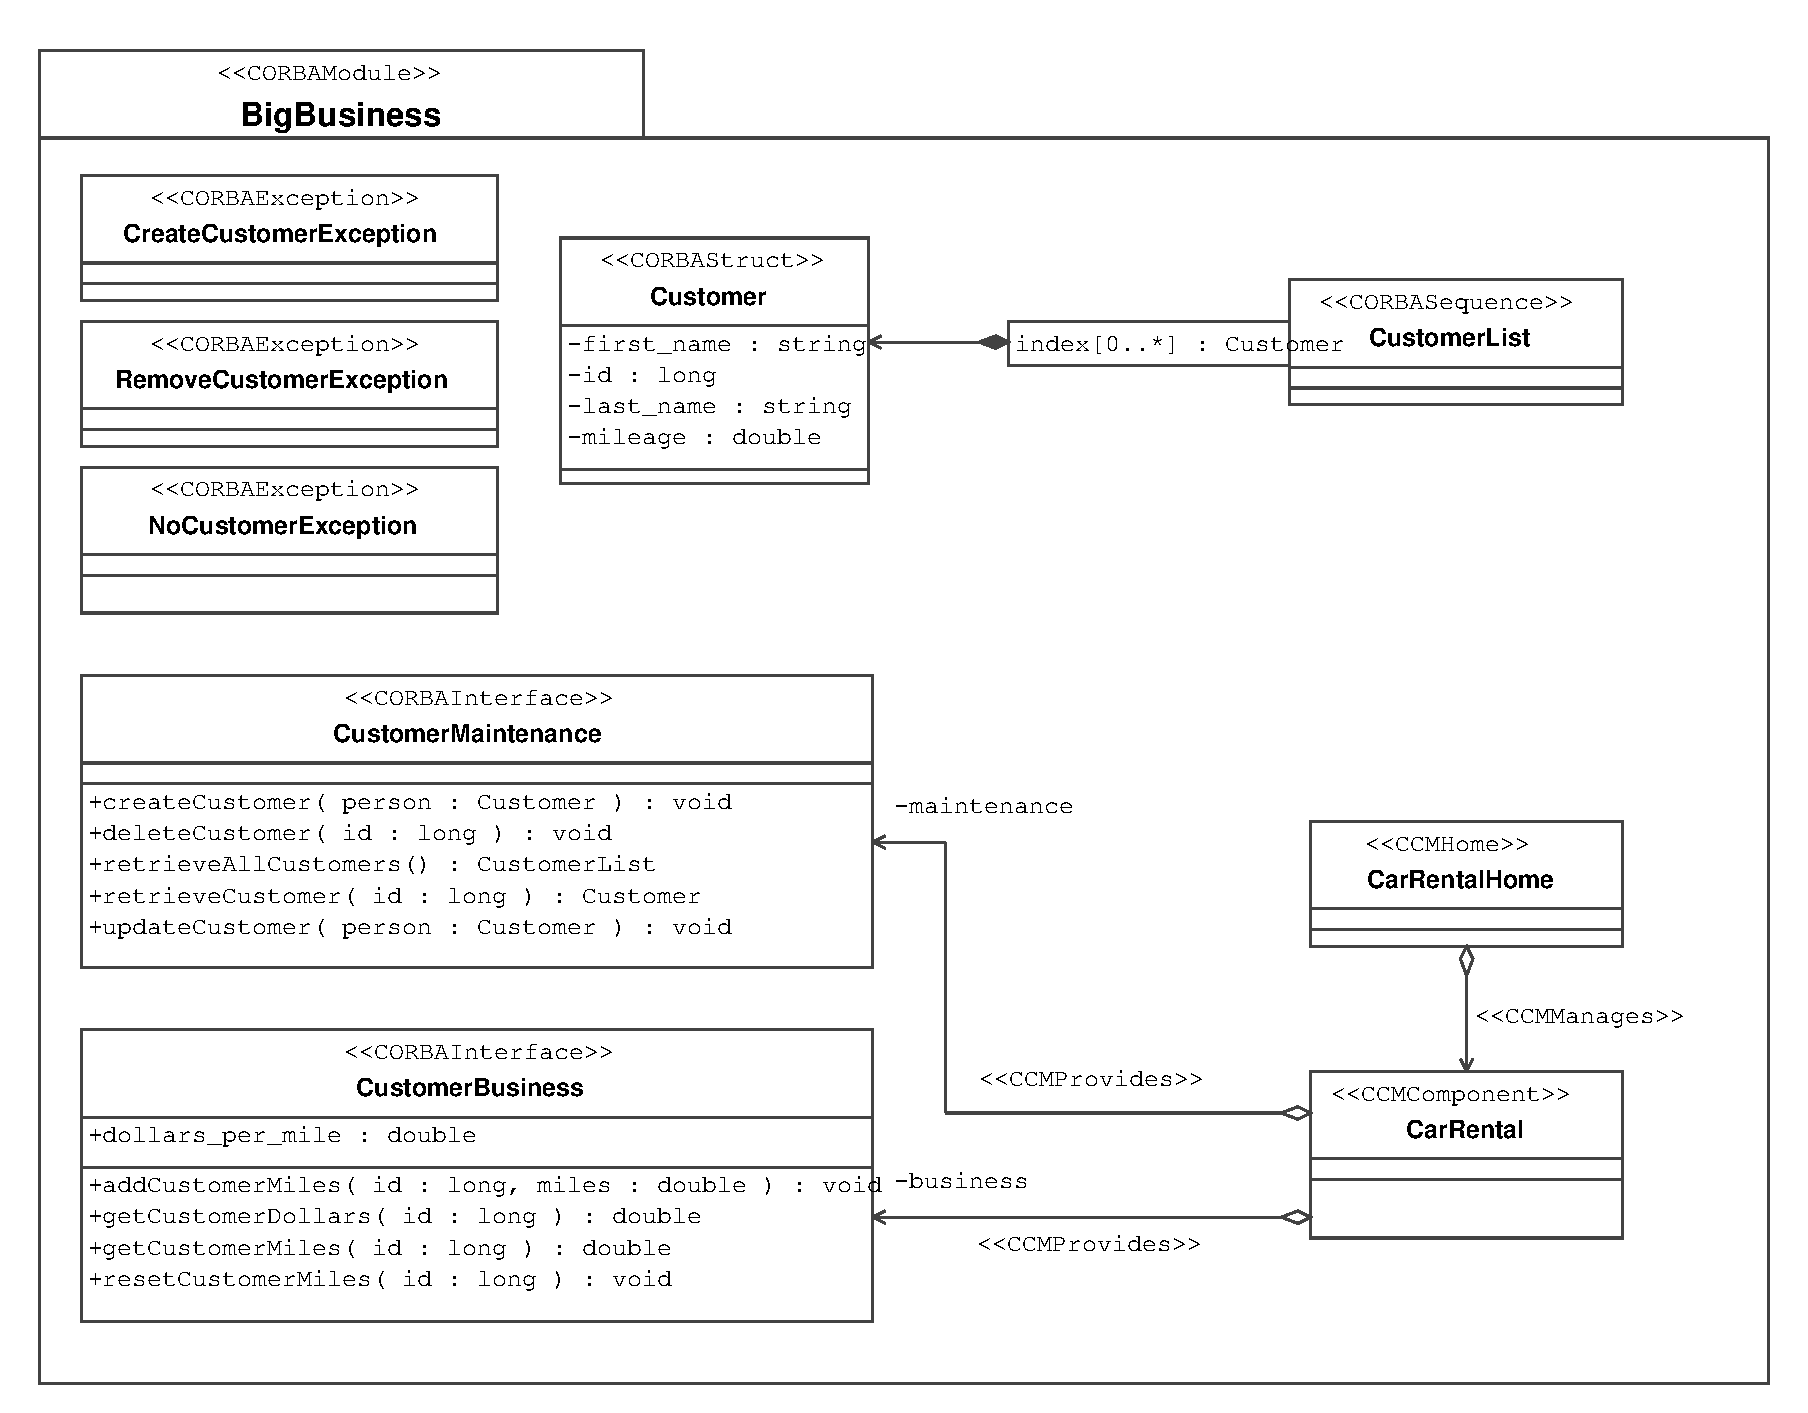
\includegraphics [width=13cm,angle=0] {uml/Example1}
        \caption{CarRental component in UML}
        \label{fig:uml-component-example}
    \end{center}
\end{figure}

We store the diagram (as an {\it XMI 1.1} file) in a directory called 
{\tt example2}, change to that directory and run the {\tt uml2idl} generator:
\begin{small}
\begin{verbatim}
    ~/example2> uml2idl uml/Example2.xml.zip example2
\end{verbatim}
\end{small}
After running {\tt uml2idl}, the new directory contains the following files:
\begin{small}
\begin{verbatim}
    example2/
    |-- example2.idl
    |-- example2.ocl
    `-- uml
        `-- Example2.xml.zip
\end{verbatim}
\end{small}

\newpage
\begin{itemize}
\item {\tt Example2.xml.zip}\\
This is the XMI file written from a UML tool.

\item {\tt example2.idl}\\ 
This file contains all generated IDL statements. 

\item {\tt example2.ocl} \\
In this file, all OCL expressions defined in the source model are stored.
Currently, we don't care about this file but we will use it in context of
Design by Contract. 
\end{itemize}

From the single IDL3 file, we generate a bunch of well structured 
IDL3 files as done with manually written files:
\begin{small}
\begin{verbatim}
    ~/example2> ccmtools-generate idl3 -o CarRental/idl3 *.idl
\end{verbatim}
\end{small}

Again, we have separated interfaces from component definitions:
\begin{small}
\begin{verbatim}
CarRental
`-- idl3
    |-- component
    |   `-- BigBusiness
    |       |-- CarRental.idl
    |       |-- CarRentalHome.idl
    |       |-- CarRentalHome_mirror.idl
    |       `-- CarRental_mirror.idl
    `-- interface
        `-- BigBusiness
            |-- CreateCustomerException.idl
            |-- Customer.idl
            |-- CustomerBusiness.idl
            |-- CustomerList.idl
            |-- CustomerMaintenance.idl
            |-- NoCustomerException.idl
            `-- RemoveCustomerException.idl
\end{verbatim}
\end{small}

That's it, we have made the first step toward MDA! 

But remember, we have only generated a component's structural description from
a UML diagram. The generated IDL file is a pure syntax description, without 
any semantics.  


%------------------------------------------------------------------------------
\section{The developers's job}
%------------------------------------------------------------------------------

It's important to know, that a developer's job does not change whether a 
component is designed in UML or IDL.
In both cases, a developer starts from the IDL3 file structure as shown above.

% $Id$
%==============================================================================
\chapter{System Development}
%==============================================================================
\begin{flushright}
{\it }
\end{flushright}

blah \dots


\newpage
% $Id$
%==============================================================================
\chapter{UML Component Design}
%==============================================================================

Remember, component based development starts with component design.
A component designer specifies components using the 
{\it Interface Definition Language} (IDL).

On the other side, the OMG proposes a {\it Model Driven Architecture} (MDA) 
where development starts at abstract levels called 
{\it Platform Independent Models} (PIM).
After some refinement steps, these PIM are transformed to 
{\it Platform Specific Models} (PSM).
Finally, from PSM, tools can generate source code that implements the modeled 
application.

OK, that's the vision. 
In practice, there are still problems in applying MDA because modeling of 
behavior is difficult (even in UML 1.x) and tool support is marginal. 
However, the MDA ideas are very interesting, thus CCM Tools make a first step 
in this direction by designing components in UML 1.4.

%------------------------------------------------------------------------------
\section{Model driven development}
%------------------------------------------------------------------------------

To design components in UML we use the {\it UML Profile for CCM} 
\cite{UML-CORBA-Profile,UML-CCM-Profile}. 
This profile is basically a class diagram using a bunch of stereotypes.
For each IDL construct there is a corresponding representation in UML class 
diagram.

\begin{figure}[htbp]
    \begin{center}
        \includegraphics [width=9cm,angle=0] {UMLComponentDesign}
        \caption{UML component design}
        \label{fig:uml-component-design}
    \end{center}
\end{figure}

A component designer paints the UML representation of components using a UML 
tool that stores diagrams in XMI 1.1 format 
(Fig.~\ref{fig:uml-component-design}).
Currently we use {\it MagicDraw} where a community edition can be downloaded 
for free).

From the stored XMI file, the {\tt uml2idl} generator creates a single IDL file.
Optionally, this IDL file can be validated and fragmented into many source files
(that are linked via include statements) by using the {\tt idl3} generator.
IDL file partitioning prevents a developer from redundant IDL definitions 
especially when processing more components at the same time.


%------------------------------------------------------------------------------
\section{The designer's job}
%------------------------------------------------------------------------------
To figure out the new tasks of a component designer, we present a concrete 
example.
Fig.~\ref{fig:uml-component-example} shows the UML representation of our first 
component definition.
The mapping from UML profile to IDL is straight forward. A UML 
package is mapped to an IDL module, UML classes are mapped to IDL constructs
corresponding to their given stereotypes (see Example \ref{example:Exceptions} 
to \ref{example:component}).
\begin{figure}[htbp]
    \begin{center}
        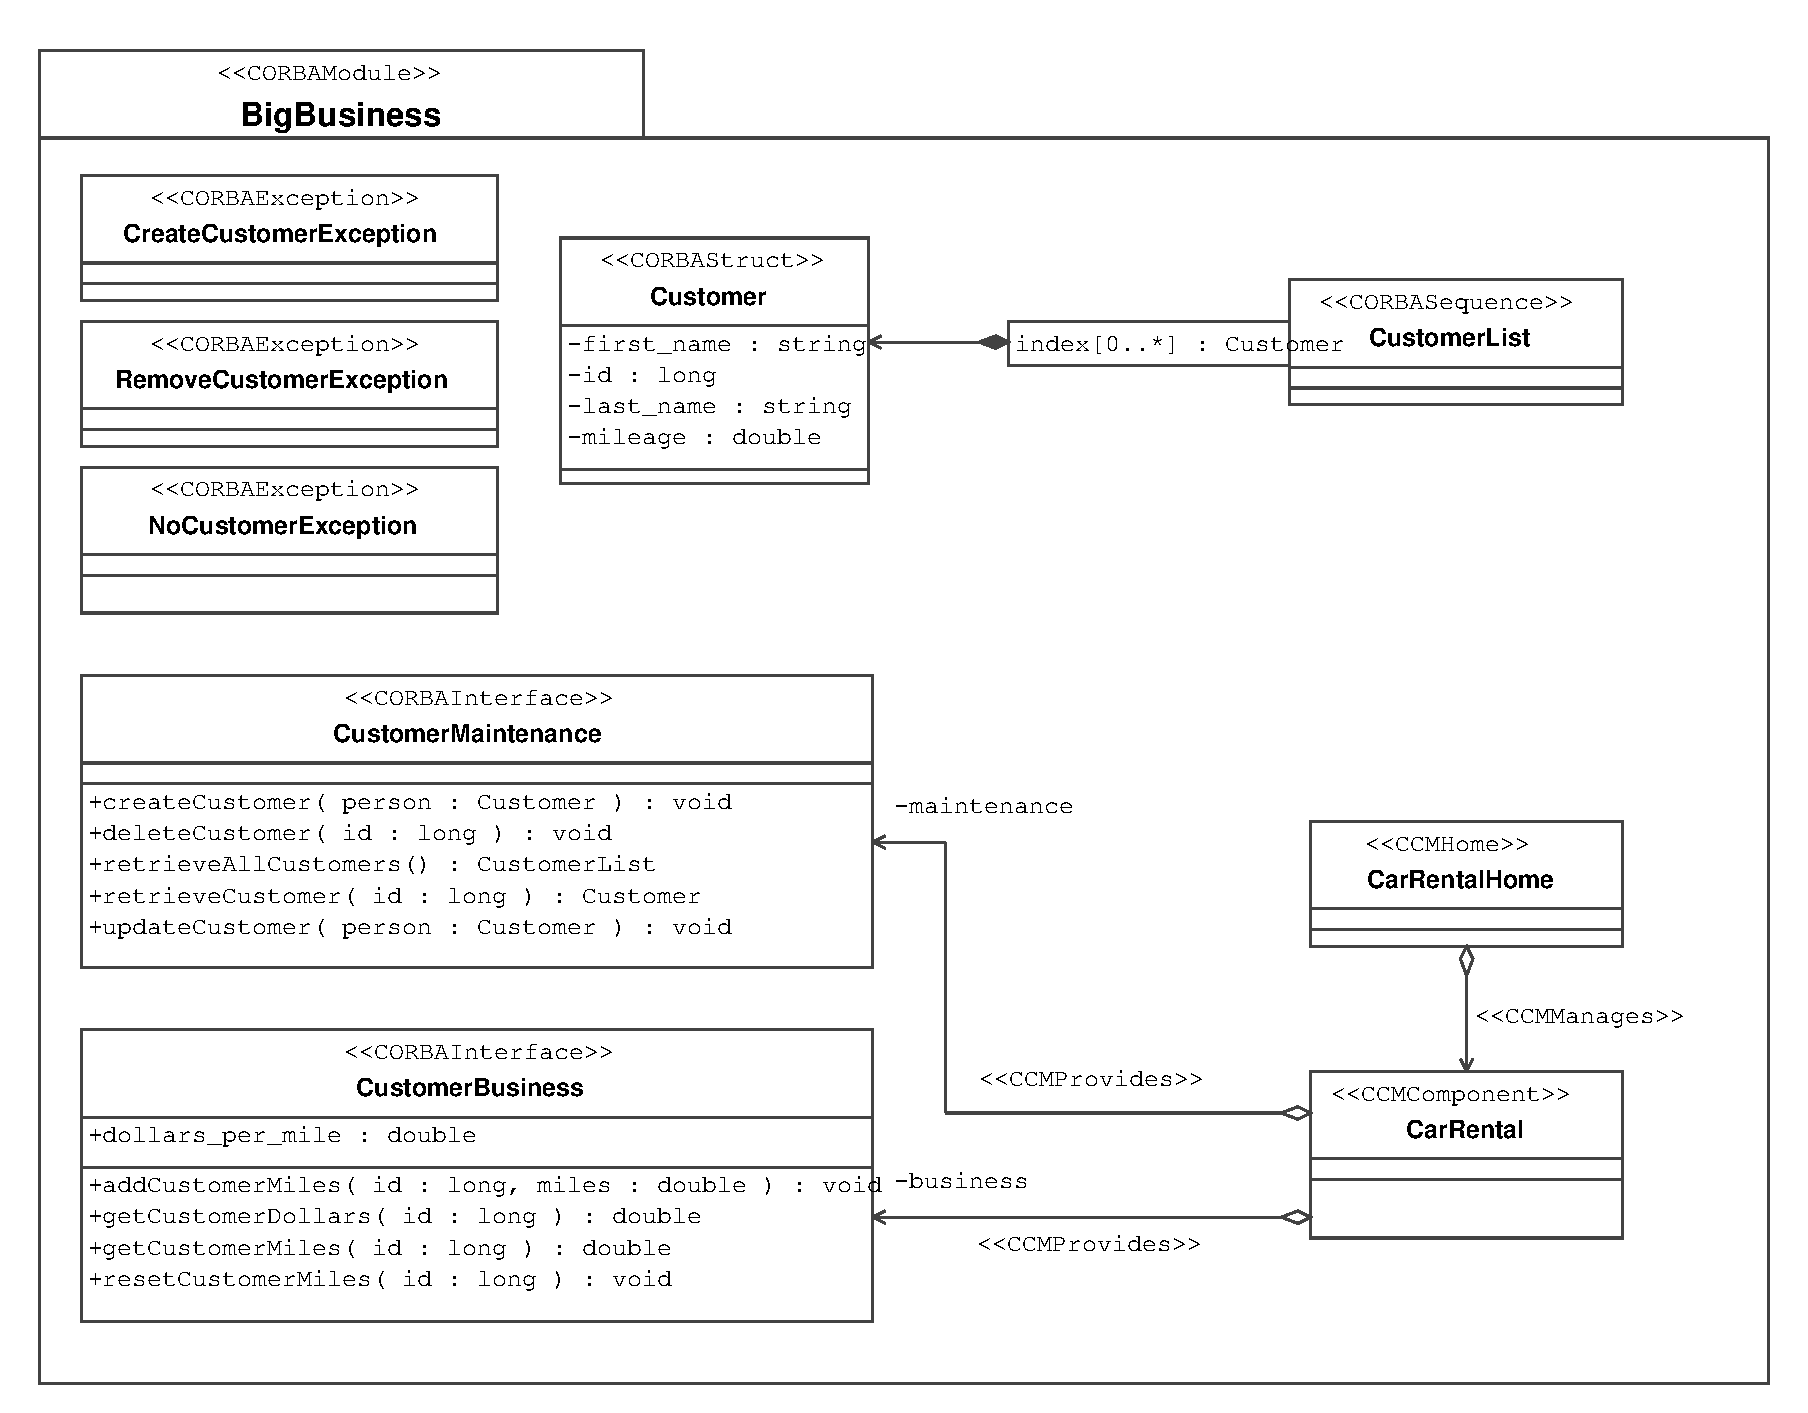
\includegraphics [width=13cm,angle=0] {uml/Example1}
        \caption{CarRental component in UML}
        \label{fig:uml-component-example}
    \end{center}
\end{figure}

We store the diagram (as an {\it XMI 1.1} file) in a directory called 
{\tt example2}, change to that directory and run the {\tt uml2idl} generator:
\begin{small}
\begin{verbatim}
    ~/example2> uml2idl uml/Example2.xml.zip example2
\end{verbatim}
\end{small}
After running {\tt uml2idl}, the new directory contains the following files:
\begin{small}
\begin{verbatim}
    example2/
    |-- example2.idl
    |-- example2.ocl
    `-- uml
        `-- Example2.xml.zip
\end{verbatim}
\end{small}

\newpage
\begin{itemize}
\item {\tt Example2.xml.zip}\\
This is the XMI file written from a UML tool.

\item {\tt example2.idl}\\ 
This file contains all generated IDL statements. 

\item {\tt example2.ocl} \\
In this file, all OCL expressions defined in the source model are stored.
Currently, we don't care about this file but we will use it in context of
Design by Contract. 
\end{itemize}

From the single IDL3 file, we generate a bunch of well structured 
IDL3 files as done with manually written files:
\begin{small}
\begin{verbatim}
    ~/example2> ccmtools-generate idl3 -o CarRental/idl3 *.idl
\end{verbatim}
\end{small}

Again, we have separated interfaces from component definitions:
\begin{small}
\begin{verbatim}
CarRental
`-- idl3
    |-- component
    |   `-- BigBusiness
    |       |-- CarRental.idl
    |       |-- CarRentalHome.idl
    |       |-- CarRentalHome_mirror.idl
    |       `-- CarRental_mirror.idl
    `-- interface
        `-- BigBusiness
            |-- CreateCustomerException.idl
            |-- Customer.idl
            |-- CustomerBusiness.idl
            |-- CustomerList.idl
            |-- CustomerMaintenance.idl
            |-- NoCustomerException.idl
            `-- RemoveCustomerException.idl
\end{verbatim}
\end{small}

That's it, we have made the first step toward MDA! 

But remember, we have only generated a component's structural description from
a UML diagram. The generated IDL file is a pure syntax description, without 
any semantics.  


%------------------------------------------------------------------------------
\section{The developers's job}
%------------------------------------------------------------------------------

It's important to know, that a developer's job does not change whether a 
component is designed in UML or IDL.
In both cases, a developer starts from the IDL3 file structure as shown above.

% $Id$ 
%==============================================================================
\section{A Nested Component's Structure}
%==============================================================================

\begin{figure}[htb]
    \begin{center}
    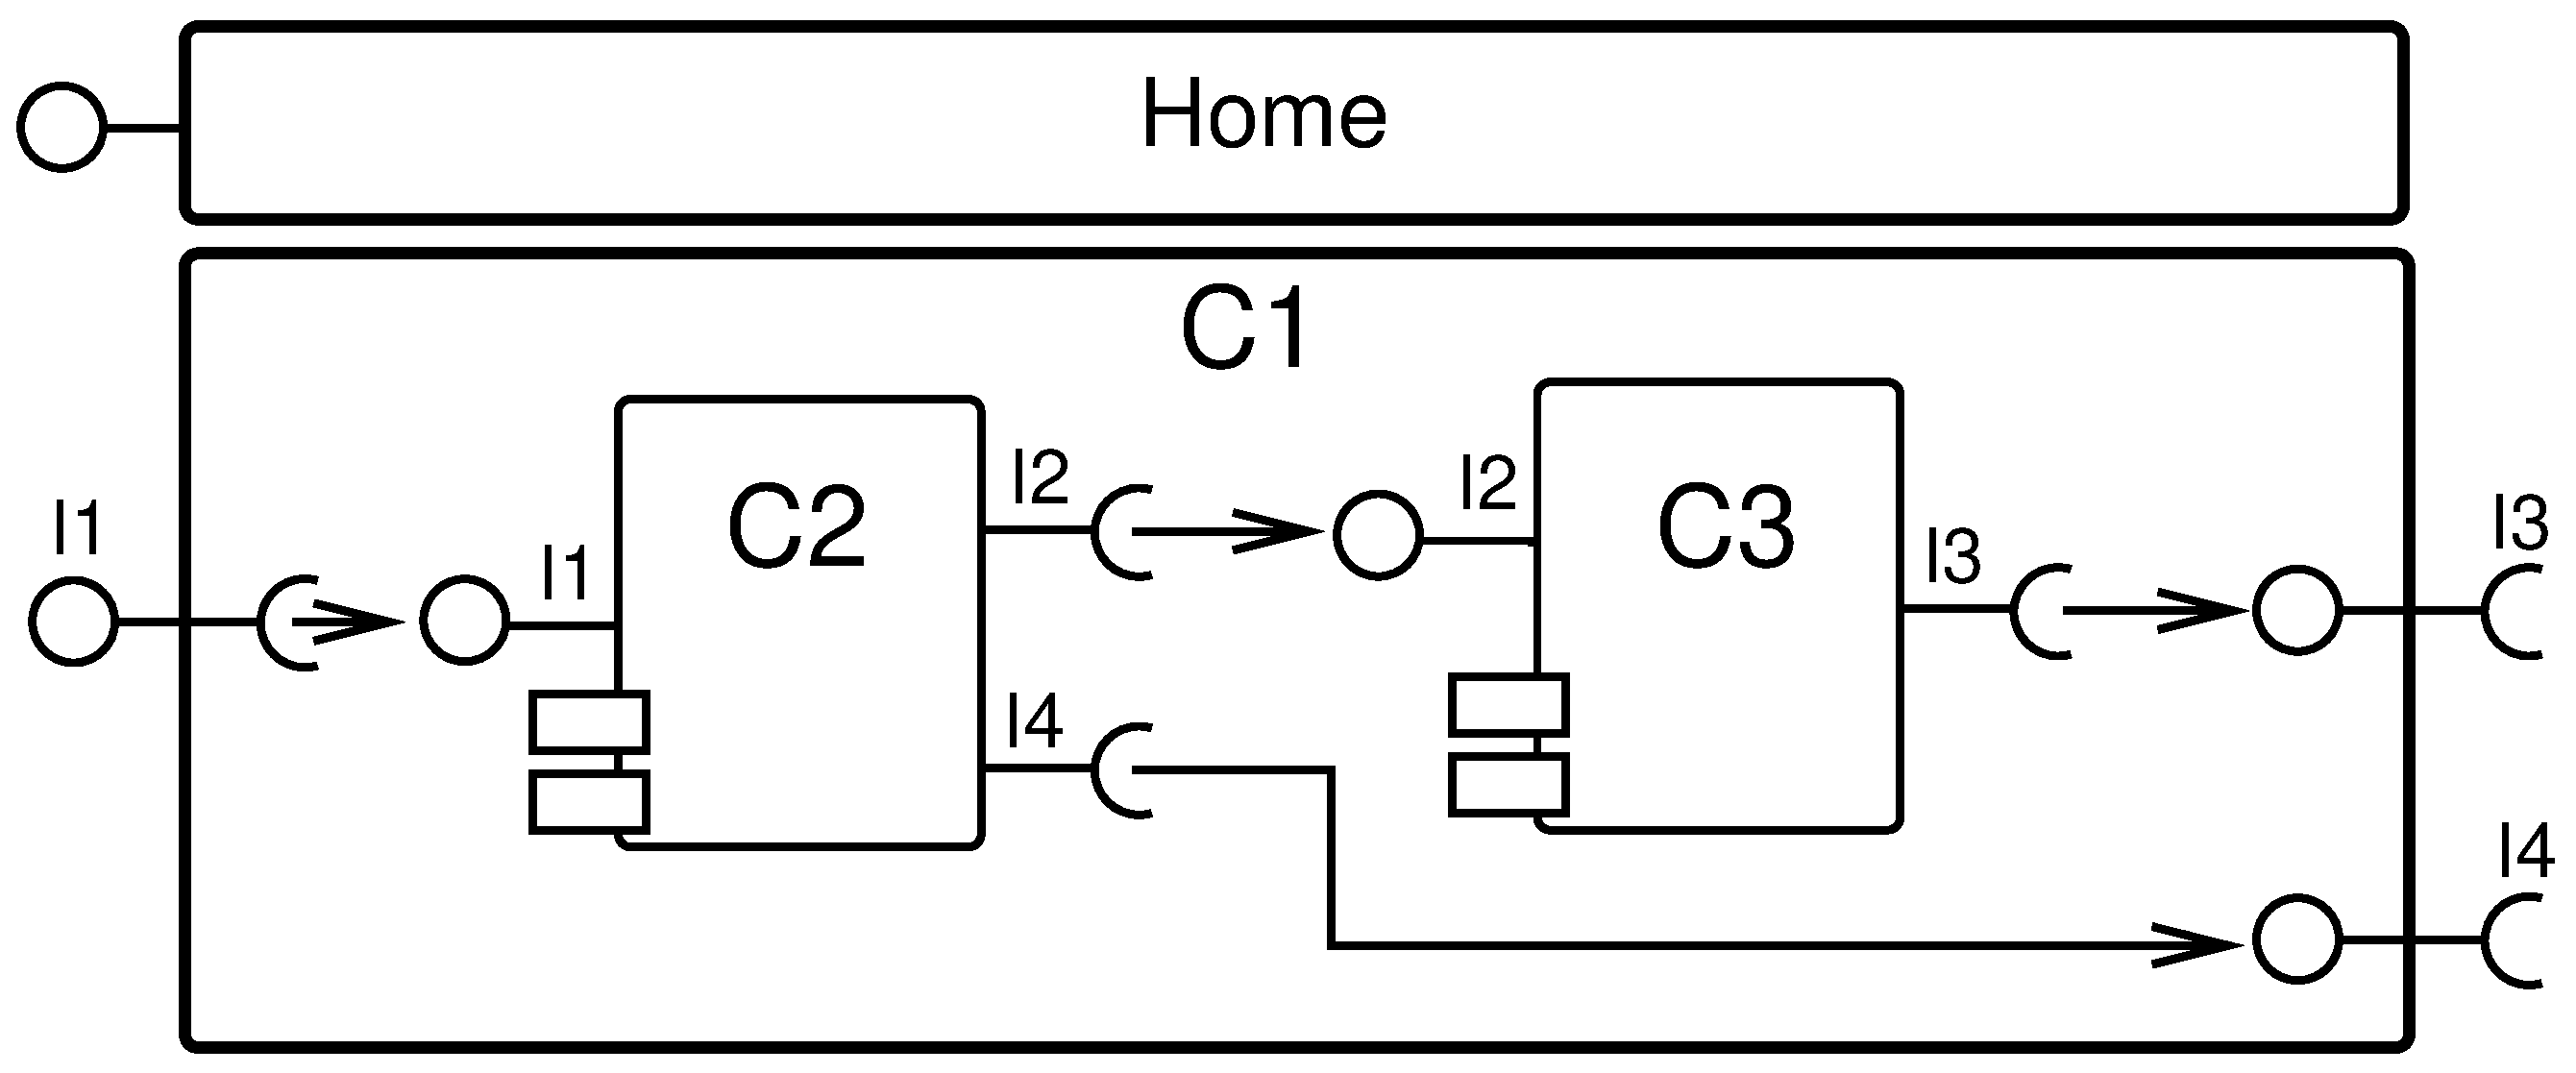
\includegraphics [width=7cm,angle=0] {figures/NestedAssembly.eps}
    \caption{ $C_{Ref}$ super component example.}
    \label{NestedAssembly}
    \end{center}
\end{figure}

Using the session facade pattern \cite{J2EECorePatterns}, 
we are able reduce a nested component composition into a flat component 
assembly that can be described by a simple CAD file.
While the inner components $C2$, $C3$ keep unchanged, the outer component $C1$ 
must be transformed into a special LwCCM component - the facade component, 
as shown in Fig.~\ref{NestedToFlatAssembly}.

\begin{figure}[htb]
    \begin{center}
    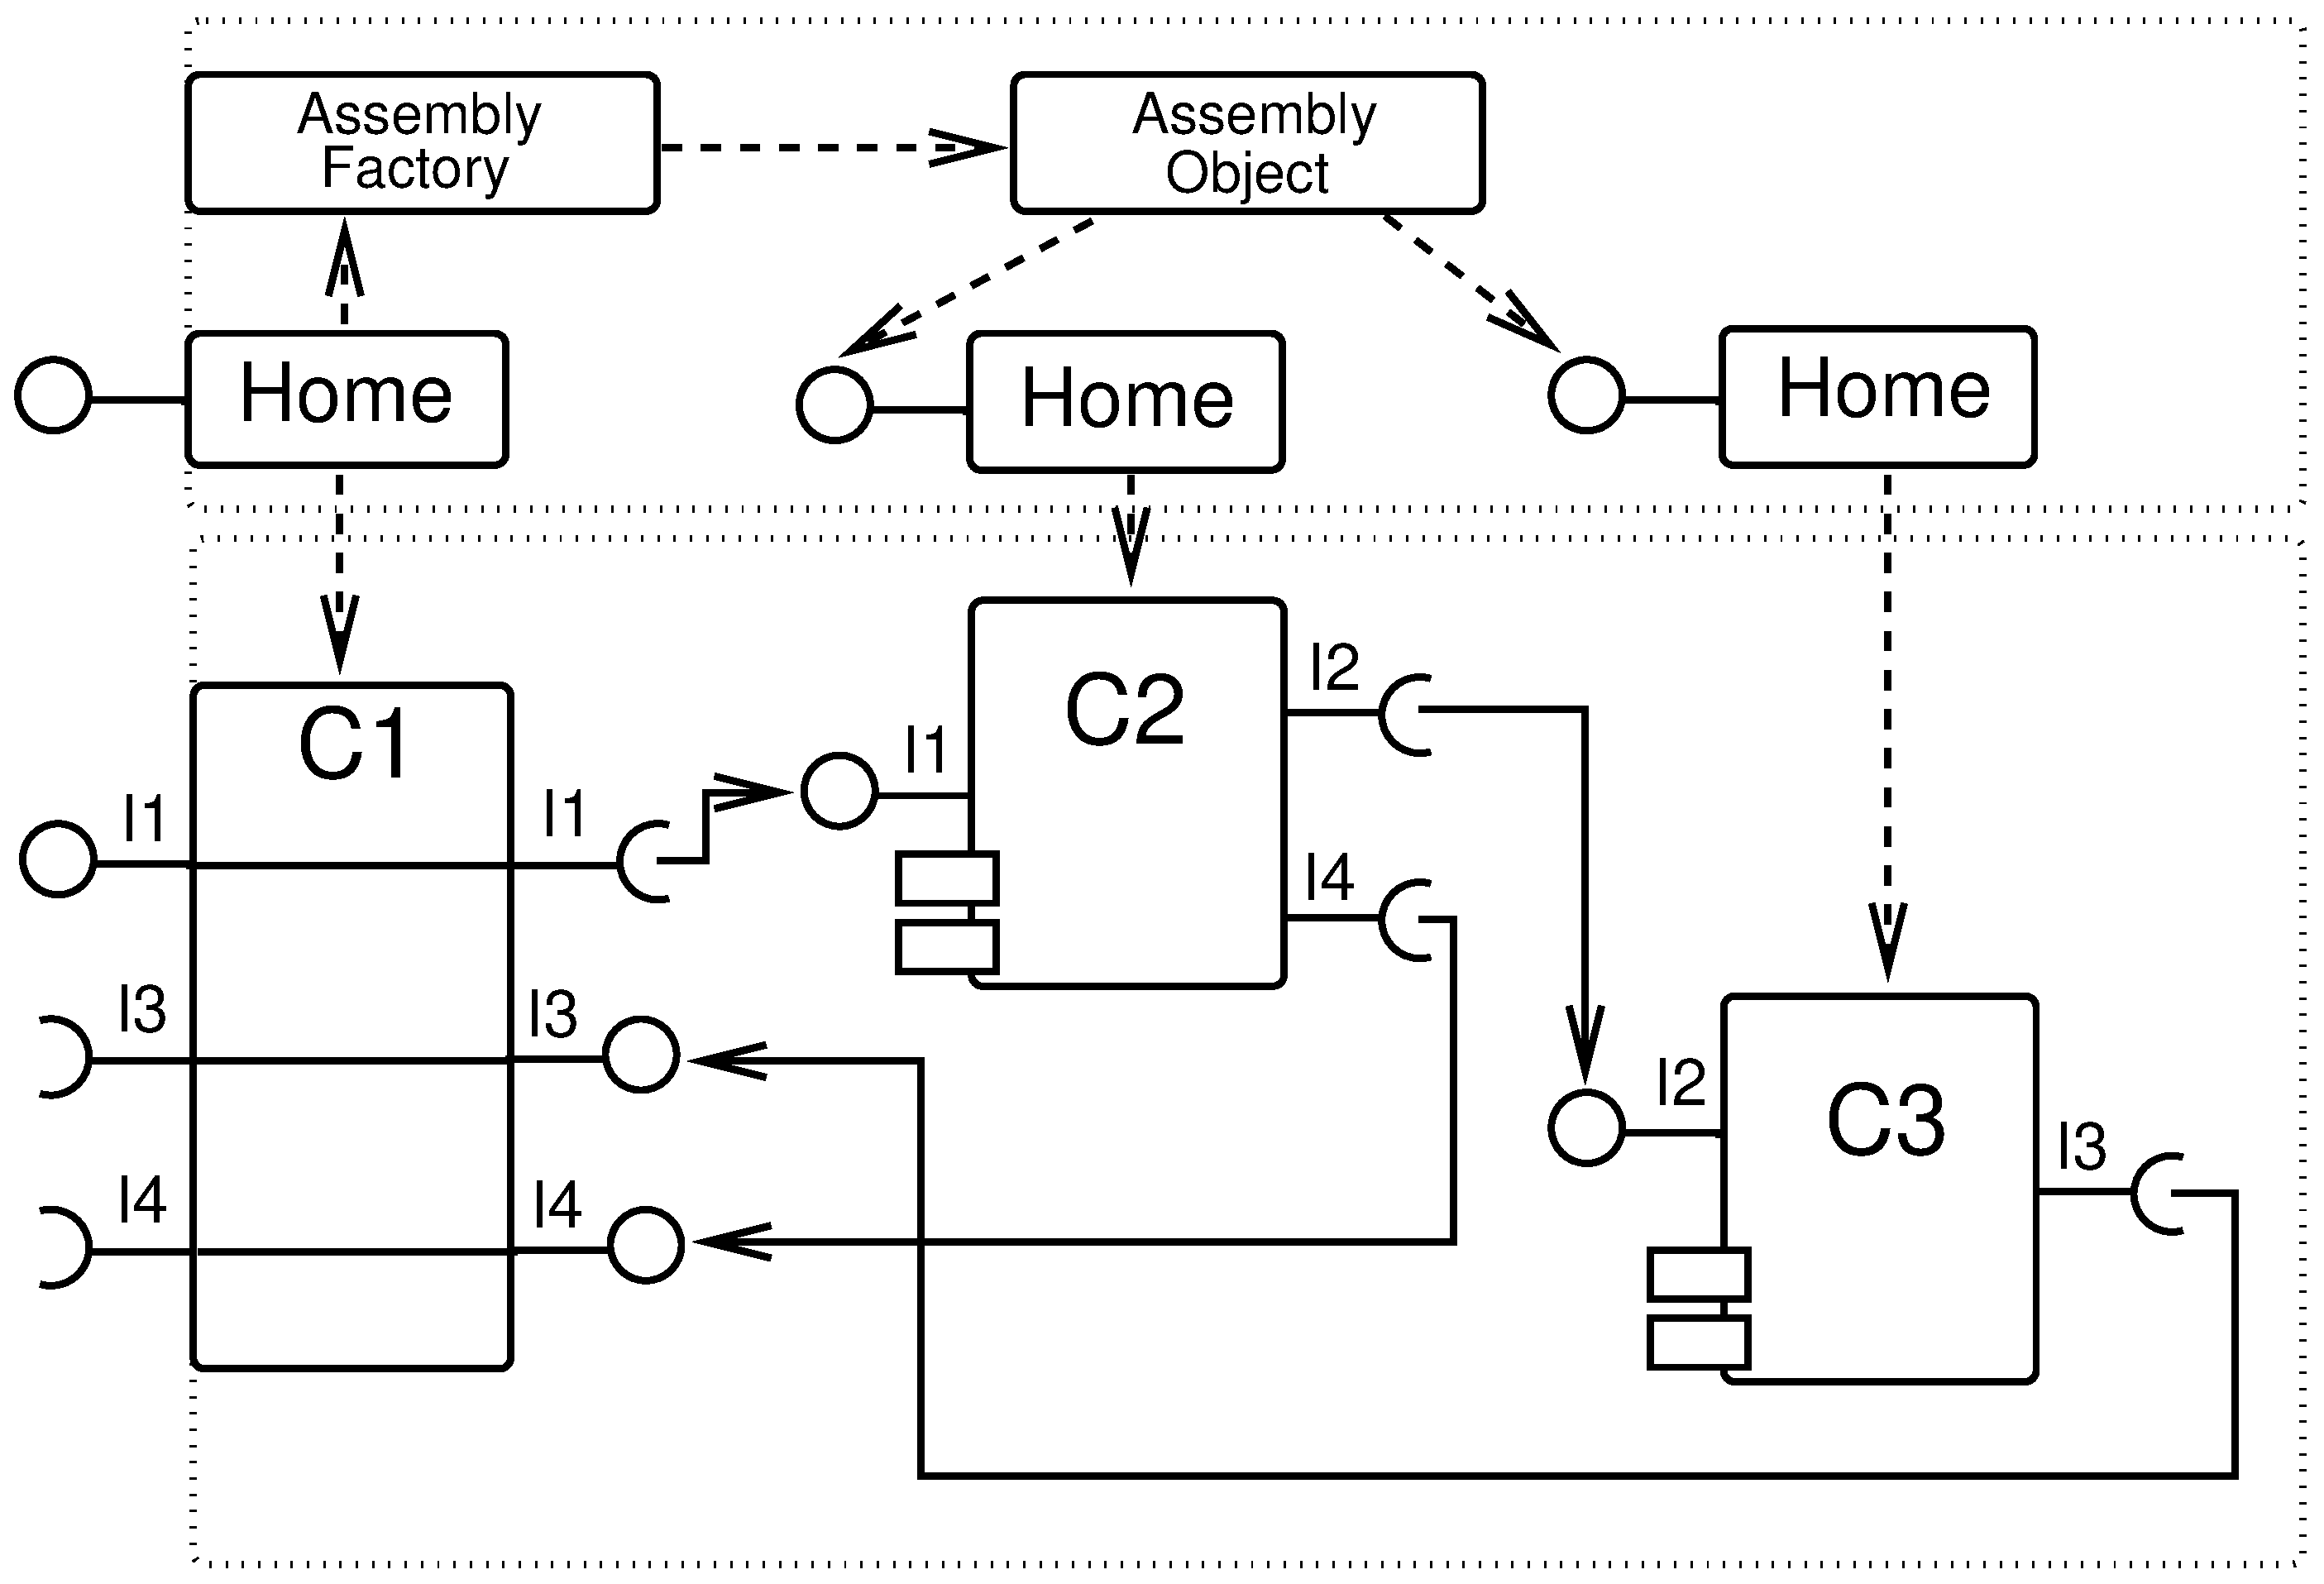
\includegraphics [width=7cm,angle=0] {figures/NestedToFlatAssembly.eps}
    \caption{Using the session facade pattern, a nested component composition
    can be reduced to a flat assembly as defined in LwCCM.}
    \label{NestedToFlatAssembly}
    \end{center}
\end{figure}

\noindent
The LwCCM facade component provides two complementary kinds of ports for each 
port defined in $C1$:
\begin{itemize}
\item {\bf Public ports.} A public port is visible to component clients and
can be accessed as a regular LwCCM component port.
 
\item {\bf Private ports.} A private port is a LwCCM port that is
not visible to component clients.
Private ports are used to connect the facade component with their inner 
component instances.
Technically, private ports are implemented like public ports, but after the
configuration phase, private ports can not be accessed by component clients. 
\end{itemize}
 
\noindent
All information about components and their connections within a super 
component are represented by an {\it Assembly Object}.
Such an assembly object is assigned to a facade component instance, and 
can be seen as a part of the facade component itself. 

For each facade component instance, an instance of the corresponding assembly
object must be created. 
To give a facade component's home the ability to create assembly object 
instances, an {\it Assembly Object Factory} must be assigned to a facade 
component home during component deployment.
With this approach, we can use regular LwCCM components and assemblies
to realize the nested component concept.

The implementation of a facade component's business logic is straightforward, 
each call to a facet method delegates to the corresponding receptacle and 
vice versa.

\vspace{3mm}
\noindent
To give a client the illusion of a single component, a facade component has to
handle some tasks behind the scenes. These are defined by the following 
sequence diagrams. 

\begin{figure}[htb]
    \begin{center}
    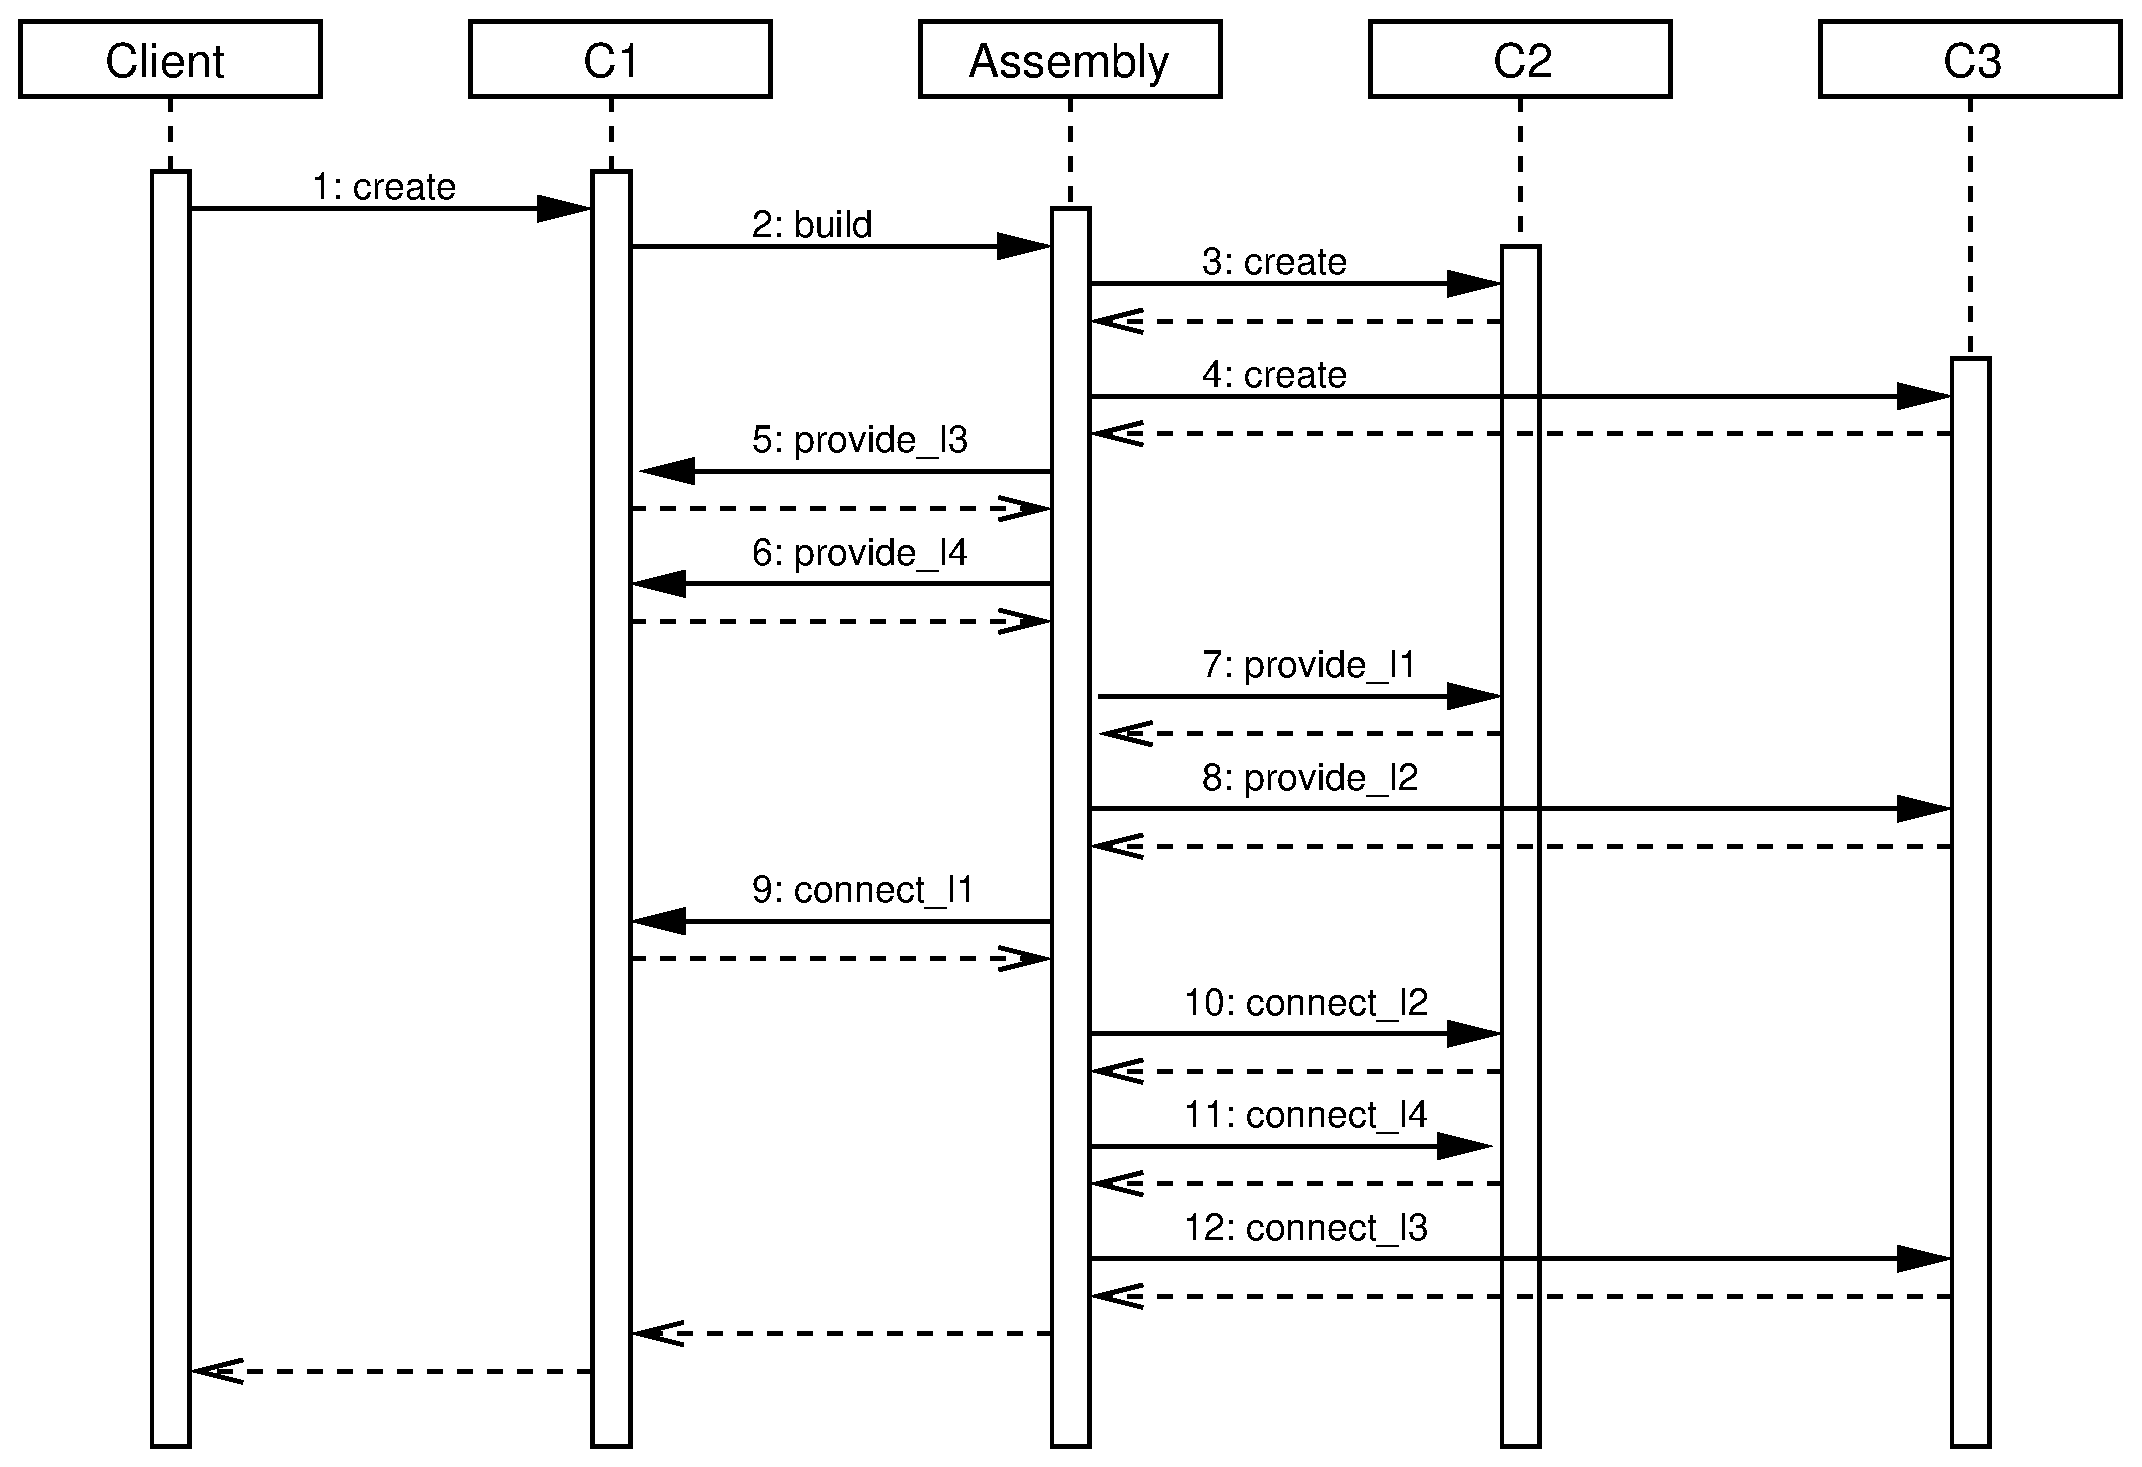
\includegraphics [width=12cm,angle=0] {figures/SuperComponentCreate.eps}
    \caption{Create a super component of Fig~\ref{NestedToFlatAssembly}.}
    \label{SuperComponentCreate}
    \end{center}
\end{figure}

\noindent
From a client's point of view, there is only one component $C_1$ that can be
instantiated by $C_1$'s home (Fig.~\ref{SuperComponentCreate}).
In fact, $C_1$ calls the {\tt build} method of the associated assembly object.
This assembly object in turn instantiates $C_2$ and $C_3$ and establishes all 
defined connections between these component instances.
After these activities, the assembly object returns to $C_1$ that finishes 
its create method.

Of course, $C_1$ itself can be part of another super component or connected 
to other components as well.
LwCCM defines the end of a component's configuration phase by calling the
{\tt configuration\_complete} method on each component instance.
In the case of a super component, this call must be delegated to all 
subcomponent instances (Fig.~\ref{SuperComponentConfigurationComplete}).
Before $C_1$ can return from {\tt configuration\_complete}, it has to lock all
private ports to prevent clients from directly accessing contained component 
instances.

\begin{figure}[htb]
    \begin{center}
    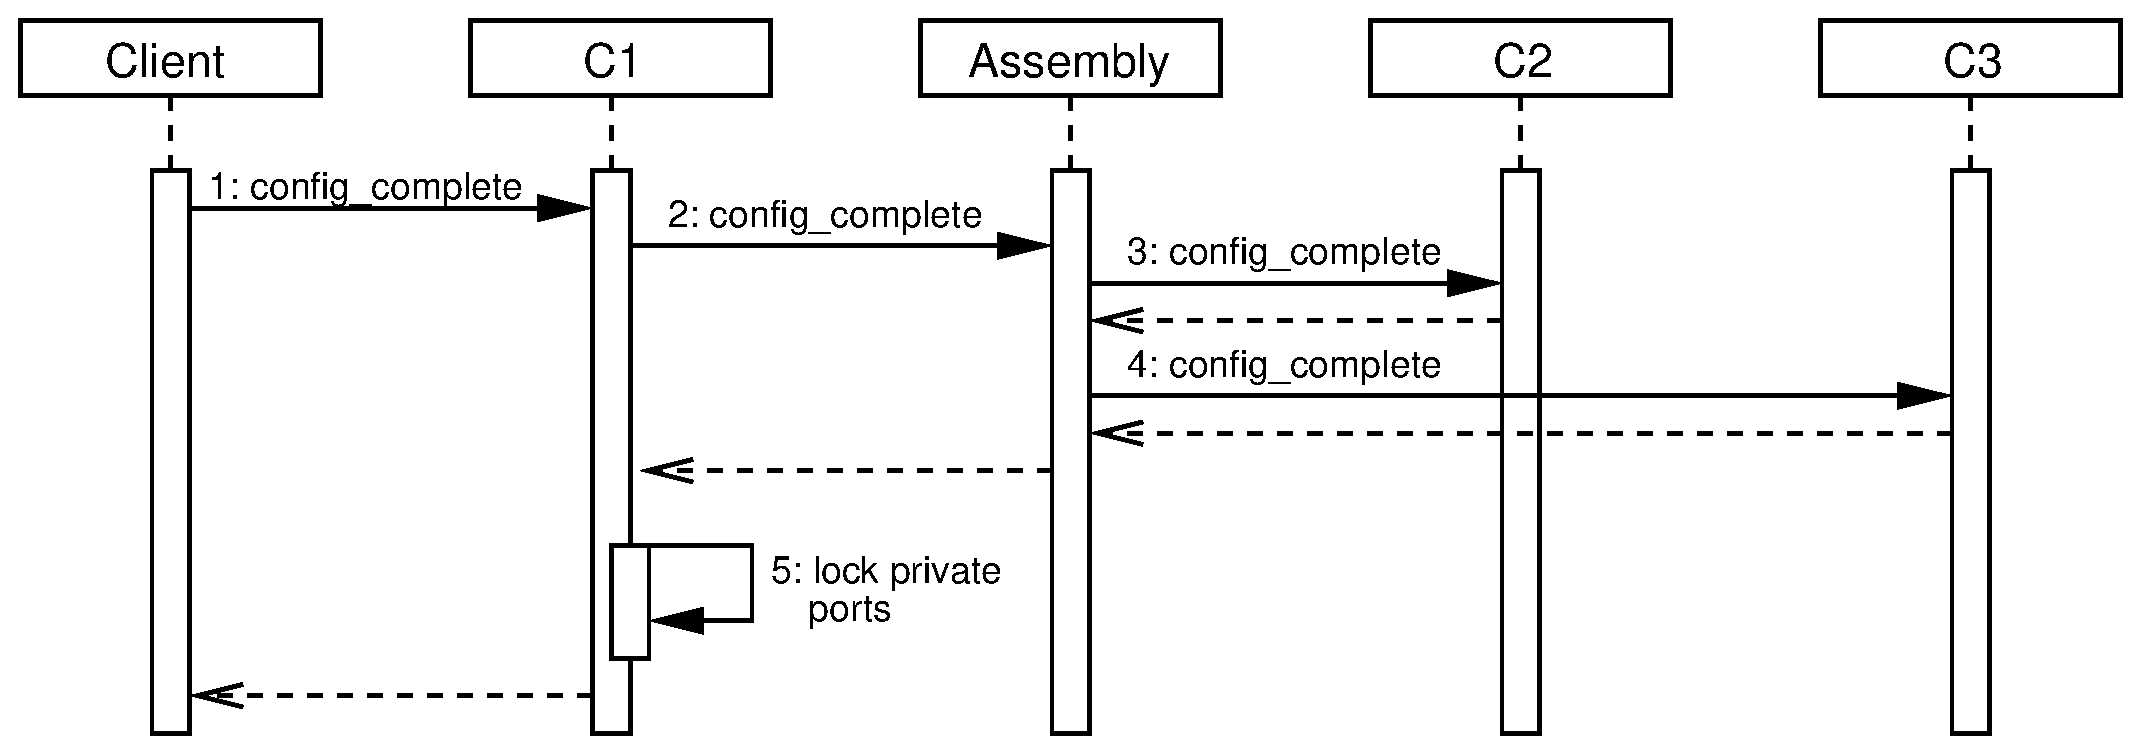
\includegraphics [width=12cm,angle=0] 
		     {figures/SuperComponentConfigurationComplete.eps}
    \caption{Completion of super component configuration phase.}
    \label{SuperComponentConfigurationComplete}
    \end{center}
\end{figure}

\noindent
Fig.~\ref{SuperComponentRemove} shows how a super component instance is removed:
$C_1$ triggers the assembly object to disconnect and destroy
all contained component instances.

\begin{figure}[htb]
    \begin{center}
    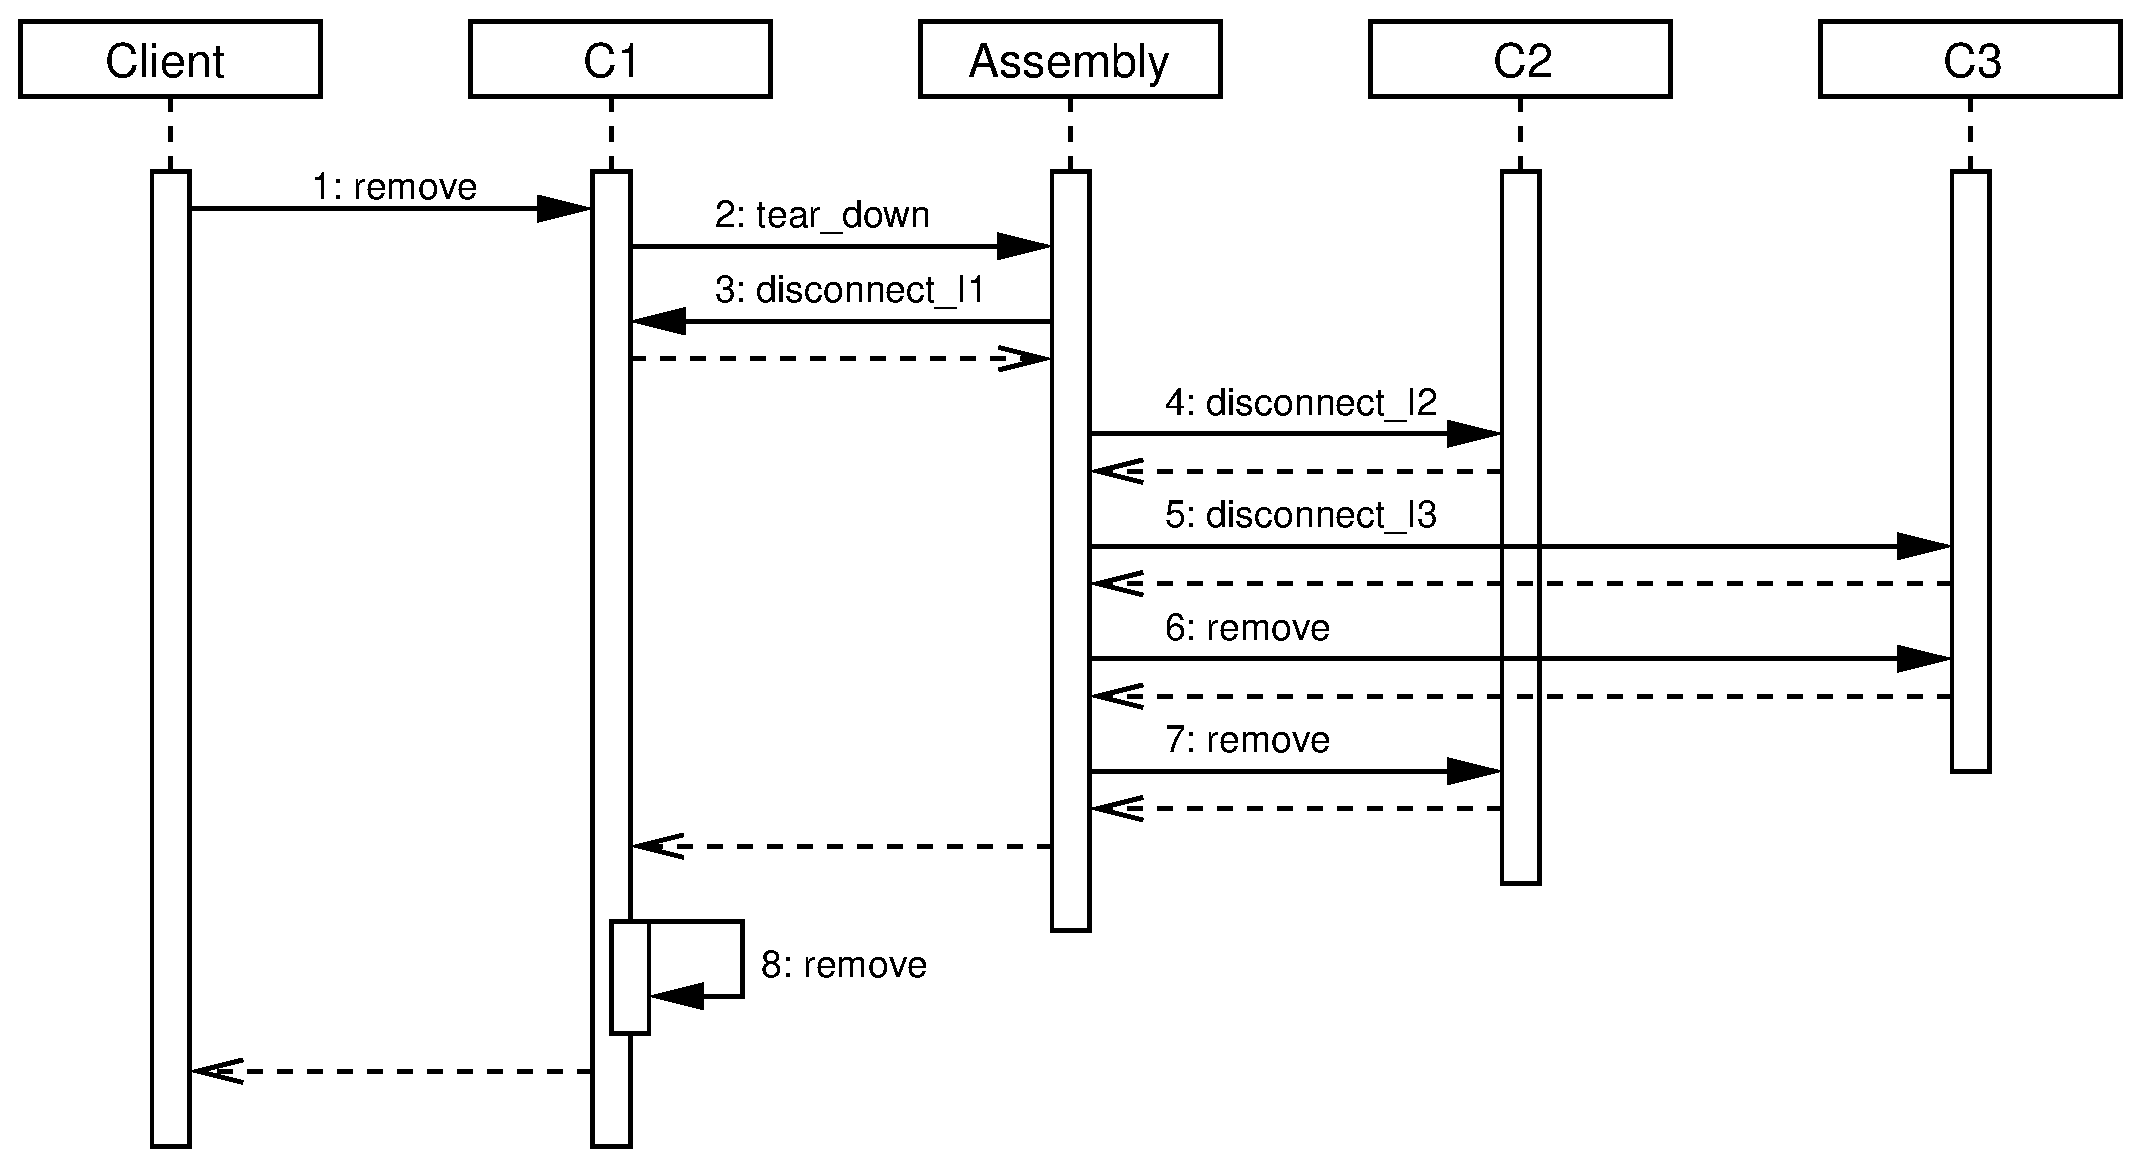
\includegraphics [width=12cm,angle=0] {figures/SuperComponentRemove.eps}
    \caption{Removal of a super component.}
    \label{SuperComponentRemove}
    \end{center}
\end{figure}

\noindent
A component client can handle
the super component in the same way as a regular LwCCM component.
Also, a simple LwCCM component can be seen as a special case of a super
component with an empty assembly.
Thus, both components and assemblies has been reduced to a single concept.


% Assemblies of components
% ModelDrivenSystemdevelopment

%% $Id$
%==============================================================================
\chapter{System Deployment}
%==============================================================================
\begin{flushright}
{\it }
\end{flushright}

blah \dots

\newpage
% $Id$

%==============================================================================
\chapter{Remote Components}
%==============================================================================

%------------------------------------------------------------------------------
\section{Overview}
%------------------------------------------------------------------------------

After implementing and using local components, let's have a look at remote
components. 
While the CCM specification describes only remote components that are
accessible from CORBA clients,  
the goal of CCM--Tools is to support local components that can be put 
transparently into remote CCM components.
You can connect remote components (generated by the CCM-Tools) with any other 
CCM components (e.g. components generated by MicoCCM).

\begin{figure}[!htb]
    \begin{center}
        \includegraphics [width=7cm,angle=0] {LCAC_Overview}
        \caption{Local component adapter}
        \label{LcacOverview}
    \end{center}
\end{figure}

\noindent
An existing local component can fit into a remote component using adapter
classes, as shown in figure \ref{LcacOverview}. For each CORBA interface
of a remote component a adapter delegates the method calls to the local 
equivalent.
To get more information about the {\bf Local Component Adapter Concept} (LCAC)
see the Appendix of this document.

%------------------------------------------------------------------------------
\section{The designer's job}
%------------------------------------------------------------------------------

Of course, developing remote CORBA components starts with an IDL file. In fact, the
IDL comes from the CORBA stuff, and has already been used for local component 
development. 
To generate a remote layer around a local component, we can use existing IDL
files.
  
\begin{Example}
\begin{minifbox}
\begin{small}
\begin{verbatim}
interface Console {
  long println(in string s);
};

component Hello {
  attribute string prompt;
  provides Console console;
};

home HelloHome manages Hello {
};
\end{verbatim}
\end{small}
\end{minifbox}
\caption{Reusing the local component's IDL definition}
\label{example:one-component-idl}
\end{Example}


%------------------------------------------------------------------------------
\section{The developer's job}
%------------------------------------------------------------------------------

The basic idea is that a component developer always implements a local component.
Business logic is implemented in respect to the local component's programming
model without any CORBA in mind (and code ;-).
Thus, we start with implementing a local component as shown before:
\begin{small}
\begin{verbatim}
~/hello> ccmtools-c++-generate -d -c 2.0 -p hello2.0 Hello.idl
~/hello> ccmtools-c++-configure -p hello2.0
~/hello> ccmtools-c++-make -p hello1.0
\end{verbatim}
\end{small}

We implement the component's test, write the business logic, run the test and so on.
Remember, this iterative programming style forces short turn around cycles that are
not possible in a pure CORBA component environment.



%------------------------------------------------------------------------------
\subsection{Set up remote component environment}
%------------------------------------------------------------------------------

The remote components need some libraries, header and IDL files to run. All these
stuff can be generated, compiled and installed, using the following script: 
\begin{small}
\begin{verbatim}
~/hello> ccmtools-c++remote-environment
\end{verbatim}
\end{small}
	
\noindent
Note that the CCM--Tools need the {\bf Mico ORB}, {\bf IDL compiler} and 
{\bf NameService} to generate, build and run remote components.

 

%------------------------------------------------------------------------------
\subsection{Create the remote layer}
%------------------------------------------------------------------------------

To add a remote layer to an existing local component, we have to generate the
CORBA stubs and remote component adapters that join the CORBA objects with the
local component implementation.
All this code is generated using the following script:

\begin{small}
\begin{verbatim}
~/hello> ccmtools-c++remote-generate -d -p hello1.0 Hello.idl
\end{verbatim}
\end{small}
The {\tt ccmtools-c++remote-generate} script accepts the following command line
parameters:
\begin{itemize}
\item {\tt -d, -\-debug }\\
Enable debugging in generated code. The generated code produces a lot of debug
messages that can be used to trace the program execution. This also causes a
test client to be generated.

\item {\tt -p NAME, -\-package=NAME}\\
Set package name to NAME. The default package name is ``ccmtools-package''. Note
that the package name is used for the name of the generated subdirectory, unless
you override this behavior with the {\tt -o} option.

\item {\tt -h, -\-help}\\
Print out a short description of the available command line parameters.
\end{itemize}


\noindent
Beside the already existing directories and files of the local component code, 
now there are some new directories that contains the code for CORBA stubs and 
the remote component adapters.
Additionally, a second test file ({\tt \_check\_CCM\_Session\_*\_remote.cc}) is
created.

\begin{small}
\begin{verbatim}
    hello/
    |-- Hello.idl
    |-- _check_CCM_Session_Hello_remote.cc
    |-- hello1.0/
    |   |-- CCM_Session_Hello_remote
    |   |-- CCM_Test
    |   |-- idl2
\end{verbatim}
\end{small}

\noindent
We can build the local component code as well as the remote code with the
following commands:
\begin{small}
\begin{verbatim}
~/hello> ccmtools-c++-configure -p hello1.0
~/hello> ccmtools-c++-make -p hello1.0
\end{verbatim}
\end{small}
After the configure and build process, the local and the remote component tests
are started.
For the remote component test we use the CORBA collocation mechanism. Thus the 
generator  can implement the server and client code in a single test file.
Remember that to run the remote test a CORBA NameService must be established.


%------------------------------------------------------------------------------
\subsection{Deploy the remote component}
%------------------------------------------------------------------------------

To install the generated remote component library and header files in the
component repository, we can use the known CCM--Tools script:
\begin{verbatim}
~/hello> ccmtools-c++-install -p hello1.0
\end{verbatim}

\noindent
Applications can use the repository to access local or remote components 
like ordinary libraries.


%------------------------------------------------------------------------------
\subsection{Write a remote client and server}
%------------------------------------------------------------------------------

A remote component must be activated within a CORBA server application that
includes the header files of the ORB, the CORBA stubs and the remote
component.
\begin{Example}
\begin{minifbox}
\begin{small}
\begin{verbatim}
#include <CORBA.h>
#include <coss/CosNaming.h>

#include <CCM_Utils/Debug.h>
#include <CCM_Remote/CCM_Session_Hello/HelloHome_remote.h>
#include <Hello.h>

using namespace std;
using namespace CCM_Utils;
\end{verbatim}
\end{small}
\end{minifbox}
\caption{CORBA and remote component header files.}
\label{ServerHeaderFiles}
\end{Example}

\noindent
The remote {\tt Hello} component can be activated using the generated {\tt deploy\_HelloHome()} 
function. The first parameter is the initialized ORB object and the second parameter
defines the name of the component's home. This name is used to register the component's
home in the CORBA NameService. 
\begin{Example}
\begin{minifbox}
\begin{small}
\begin{verbatim}
int main (int argc, char *argv[])
{
  // Set debugging mode
  Debug::set_global(true); 

  // Initialize ORB and value type factories
  CORBA::ORB_var orb = CORBA::ORB_init(argc, argv);
  CCM::register_all_factories (orb);

  int error = deploy_HelloHome(orb, "HelloHome:1.0");
  if(!error) {
    cout << "Component is running..." << endl;
  }
  else {
    cerr << "ERROR: Can't start components!" << endl;
    assert(0);
  }

  // Wait for CORBA requests
  orb.run();
}
\end{verbatim}
\end{small}
\end{minifbox}
\caption{Remote component activation.}
\label{RemoteComponentServer}
\end{Example}

\noindent
Note that the ORB must be initialized and started before a remote component
can be accessed from a CORBA client.

\noindent
The remote client also has to initialize the ORB and the CORBA NameService,
as shown in Example \ref{ClientInit}.
\begin{Example}
\begin{minifbox}
\begin{small}
\begin{verbatim}
int main (int argc, char *argv[])
{
  Debug::set_global(true); 

  // Initialize ORB 
  CORBA::ORB_var orb = CORBA::ORB_init(argc, argv);
  CORBA::Object_var obj = 
    orb->resolve_initial_references ("NameService");
  CosNaming::NamingContextExt_var nc = 
    CosNaming::NamingContextExt::_narrow (obj);
\end{verbatim}
\end{small}
\end{minifbox}
\caption{Initialize the client's ORB and NameService.}
\label{ClientInit}
\end{Example}

From the CORBA NameService, the client gets a reference to the 
remote component's home. 
After narrowing the CORBA reference to the particular home type, 
the {\tt create()} method is used to get a component instance.
From the component instance we get a {\tt Console} facet reference, 
and set the {\tt prompt} attribute. 
A {\tt configuration\_complete()} call finishes the component 
configuration.

\begin{Example}
\begin{minifbox}
\begin{small}
\begin{verbatim}
  // Find ComponentHomes in the Naming-Service
  obj = nc->resolve_str ("HelloHome:1.0");
  HelloHome_var myHelloHome = HelloHome::_narrow (obj);

  // Create component instances
  Hello_var myHello =  myHelloHome->create();

  // Provide facets   
  Console_var console = myHello->provide_console();
	
  // Configure the component's attribute
  myHello->prompt("=->");

  // Component configuration finished	
  myHello->configuration_complete();
\end{verbatim}
\end{small}
\end{minifbox}
\caption{Creating the remote component and facet.}
\label{CreatingRemoteComponent}
\end{Example}

\noindent 
Now the remote client can use the component instance to call methods on
the component's equivalent interface and the supported facet.
%Every client request is forwarded to a CORBA object on the server side
%that workes as an adapter to the local component implementation. 
\begin{Example}
\begin{minifbox}
\begin{small}
\begin{verbatim}
  // Call operations on the component and its facets
  cout << "Version = " << 
    myHello->getComponentVersion() << endl;
  cout << "Date = " << 
    myHello->getComponentDate() << endl;

  console->println("Hello from the remote client");
\end{verbatim}
\end{small}
\end{minifbox}
\caption{Calling the remote component methods.}
\label{RemoteMethodCalling}
\end{Example}

\noindent
Finally, the remote client removes the component instance on the server side
and exits from the main function.

\begin{Example}
\begin{minifbox}
\begin{small}
\begin{verbatim}
  // Destroy component instances
  myHello->remove();
}
\end{verbatim}
\end{small}
\end{minifbox}
\caption{Destroy component instance.}
\label{DestroyComponent}
\end{Example}



%------------------------------------------------------------------------------
\subsection{Undeploy the remote component}
%------------------------------------------------------------------------------

To remove the component's libraries and header files from the repository, 
call:
\begin{verbatim}
~/hello> ccmtools-c++-uninstall -p hello1.0
\end{verbatim}
Remember, only the installed libraries and header files are deleted while
the developers source code remains untouched.



%------------------------------------------------------------------------------
%\subsection{Remote component packaging}
%------------------------------------------------------------------------------




\begin{appendix}
%$Id$

%==============================================================================
\chapter{CCM Tools Commands}
%==============================================================================

%------------------------------------------------------------------------------
\section{ccmtools-generate}
%------------------------------------------------------------------------------

\begin{description}

\item [NAME:] 
  {\tt ccmtools-generate} - Frontend to start available CCM Tools generators.

\item [SYNOPSIS:] 
  {\tt ccmtools-generate TYPE [OPTIONS] FILES}

\item [DESCRIPTION:]
The {\tt ccmtools-generate} script is used to run a particular component generator 
backend based on a set of IDL files. 
Depending on {\tt TYPE} and {\tt OPTIONS} a particular code generator is selected 
to create the desired output.

\item [TYPE:]
  Currently, the following generator types are supported:
  \begin{itemize}
  \item {\tt c++local}\\
    Generates local C++ component logic.
    
  \item {\tt c++local-test} \\
    Generates a test client for a pair of local C++ component and
    mirror component.
    
  \item {\tt c++dbc} \\
    Generates a set of Design by Contract adapters for a local
    C++ component.
    
  \item {\tt idl3 }\\
    Generates IDL3 source files.

  \item {\tt idl3mirror }\\
    Generates IDL3 source files for a mirror component.
    
  \item {\tt idl2} \\
    Generates equivalent IDL2 source files.

  \item {\tt c++remote} \\ 
    Generates a set of remote C++ adapters that establish a standard
    compliant CORBA component where a local C++ component can be embedded.

  \item {\tt c++remote-test}\\
    Generates a test client for a pair of remote component and mirror component.
  \end{itemize}
  
\item [OPTIONS:]
  In addition to the generator types, the {\tt ccmtools-generate} script handles
  the following options:
  \begin{itemize}
  \item {\tt -a, --application} \\
    Forces the local C++ generator to create business logic
    implementation skeletons ({\tt *\_app.*} files).

  \item {\tt -h, --help} \\
    Prints out a short description of the available command line parameters.

  \item {\tt -Ipath} \\
    Specifies a path that will be handled from a preprocessor to find 
    included IDL files.

  \item {\tt -o DIR, --output=DIR} \\
    Specifies the directory where the generated code will be written. 

  \item {\tt -V, --version} \\
    Prints out the current version of installed CCM Tools.
  \end{itemize}
  
\item [FILES:]
  This {\tt ccmtools-generate} script can handle single IDL files or a list of IDL
  files. The following examples show the usage of IDL files: 
  \begin{verbatim}
    ccmtools-generate idl3mirror -o test/idl3mirror Test.idl
    ccmtools-generate c++local -a -o test Test.idl Helper.idl 
    ccmtools-generate c++local-test -o test *.idl
  \end{verbatim}

\item [SEE ALSO:]
  {\tt ccmtools-c++-generate}
  
\end{description}


%------------------------------------------------------------------------------
\section{ccmtools-c++-generate}
%------------------------------------------------------------------------------
\begin{description}

\item [NAME:] 
  {\tt ccmtools-c++-generate} - Run a sequence of generator calls.

\item [SYNOPSIS:] 
  {\tt ccmtools-C++-generate [OPTIONS] FILES}

\item [DESCRIPTION:]
  The {\tt ccmtools-c++-generate} script collects a sequence of 
  generator calls. 
  Thus, this script makes component development more convenient,
  but less flexible.   


\item [OPTIONS:]
  The {\tt ccmtools-c++-generate} script handles the following options:
  \begin{itemize}
  \item {\tt -a, --application} \\
    Forces the local C++ generator to create business logic
    implementation skeletons ({\tt *\_app.*} files).

  \item {\tt -d, --development} \\
    Using this option, for a given IDL a component, its mirror component
    and a test client will be generated.

  \item {\tt -h, --help} \\
    Prints out a short description of the available command line parameters.

  \item {\tt -Ipath} \\
    Specifies a path that will be handled from a preprocessor to find 
    included IDL files.

  \item {\tt -p NAME, --package=NAME} \\
    Specifies the directory where the generated code will be written. 
    This directory is also a package in terms of Confix.  

  \item {\tt -V, --version} \\
    Prints out the current version of installed CCM Tools.
  \end{itemize}
  
\item [FILES:]
  This {\tt ccmtools-c++-generate} script can handle single IDL files or a list of IDL
  files. The following examples show the usage of IDL files: 
  \begin{verbatim}
    ccmtools-c++-generate idl3mirror -o test/idl3mirror Test.idl
    ccmtools-generate c++local -a -o test Test.idl Helper.idl 
    ccmtools-generate c++local-test -o test *.idl
  \end{verbatim}

\item [SEE ALSO:]
  {\tt ccmtools-generate}
  
\end{description}


%------------------------------------------------------------------------------
\section{ccmtools-c++-configure}
%------------------------------------------------------------------------------
\begin{description}

\item [NAME:] 
  {\tt ccmtools-c++-configure} - Run Confix to configure the generated code.

\item [SYNOPSIS:] 
  {\tt ccmtools-C++-configure OPTION}

\item [DESCRIPTION:]
  The {\tt ccmtools-c++-configure} script is a Confix wrapper, and
  represents the following Confix call:
  \begin{small}
  \begin{verbatim}
  confix.py  --packageroot=NAME --profile="ccmtools" \
             --bootstrap --configure --quiet
  \end{verbatim}
  \end{small}
  This script makes component development more convenient,
  but less flexible. 

\item [OPTION:]
  The {\tt ccmtools-c++-configure} script needs one of the following options:
  \begin{itemize}
  \item {\tt -h, --help} \\
    Prints out a short description of the available command line parameters.

  \item {\tt -p NAME, --package=NAME} \\
    Specifies the Confix package we want to configure. 

  \item {\tt -V, --version} \\
    Prints out the current version of installed CCM Tools.
  \end{itemize}
  
\item [SEE ALSO:]
  {\tt Confix manual}
  
\end{description}


%------------------------------------------------------------------------------
\section{ccmtools-c++-make}
%------------------------------------------------------------------------------
\begin{description}

\item [NAME:] 
  {\tt ccmtools-c++-make} - Run Confix to build the generated code.

\item [SYNOPSIS:] 
  {\tt ccmtools-C++-make OPTION}

\item [DESCRIPTION:]
  The {\tt ccmtools-c++-make} script is a Confix wrapper and
  represents the following Confix call:
  \begin{small}
  \begin{verbatim}
  confix.py  --packageroot=NAME --profile="ccmtools" \
             --make --targets="all check" --quiet    
  \end{verbatim}
  \end{small}
  This script makes component development more convenient,
  but less flexible. 

\item [OPTION:]
  The {\tt ccmtools-c++-make} script needs one of the following options:
  \begin{itemize}
  \item {\tt -h, --help} \\
    Prints out a short description of the available command line parameters.

  \item {\tt -p NAME, --package=NAME} \\
    Specifies the Confix package we want to build. 

  \item {\tt -V, --version} \\
    Prints out the current version of installed CCM Tools.
  \end{itemize}
  
\item [SEE ALSO:]
  {\tt Confix manual}
  
\end{description}


%------------------------------------------------------------------------------
\section{ccmtools-c++-install}
%------------------------------------------------------------------------------
\begin{description}

\item [NAME:] 
  {\tt ccmtools-c++-install} - Run Confix to install the generated code.

\item [SYNOPSIS:] 
  {\tt ccmtools-C++-install OPTION}

\item [DESCRIPTION:]
  The {\tt ccmtools-c++-install} script is a Confix wrapper and
  represents the following Confix call:
  \begin{small}
  \begin{verbatim}
   confix.py  --packageroot=NAME --profile="ccmtools" \
              --make --targets="install" --quiet
  \end{verbatim}
  \end{small}
  This script makes component development more convenient,
  but less flexible. 

\item [OPTION:]
  The {\tt ccmtools-c++-install} script needs one of the following options:
  \begin{itemize}
  \item {\tt -h, --help} \\
    Prints out a short description of the available command line parameters.

  \item {\tt -p NAME, --package=NAME} \\
    Specifies the Confix package we want to install. 

  \item {\tt -V, --version} \\
    Prints out the current version of installed CCM Tools.
  \end{itemize}
  
\item [SEE ALSO:]
  {\tt Confix manual}
  
\end{description}



%------------------------------------------------------------------------------
\section{ccmtools-c++-uninstall}
%------------------------------------------------------------------------------

\begin{description}

\item [NAME:] 
  {\tt ccmtools-c++-uninstall} - Run Confix to uninstall the generated code.

\item [SYNOPSIS:] 
  {\tt ccmtools-C++-uninstall OPTION}

\item [DESCRIPTION:]
  The {\tt ccmtools-c++-uninstall} script is a Confix wrapper and
  represents the following Confix call:
  \begin{small}
  \begin{verbatim}
   confix.py  --packageroot=NAME --profile="ccmtools" \
              --make  --targets="uninstall distclean" --quiet
  \end{verbatim}
  \end{small}
  This script makes component development more convenient,
  but less flexible. 

\item [OPTION:]
  The {\tt ccmtools-c++-uninstall} script needs one of the following options:
  \begin{itemize}
  \item {\tt -h, --help} \\
    Prints out a short description of the available command line parameters.

  \item {\tt -p NAME, --package=NAME} \\
    Specifies the Confix package we want to uninstall. 

  \item {\tt -V, --version} \\
    Prints out the current version of installed CCM Tools.
  \end{itemize}
  
\item [SEE ALSO:]
  {\tt Confix manual}
  
\end{description}


%------------------------------------------------------------------------------
\section{ccmtools-idl}
%------------------------------------------------------------------------------

\begin{description}

\item [NAME:] 
  {\tt ccmtools-idl} - Run an IDL compiler to generate CORBA stub and skeletons.

\item [SYNOPSIS:] 
  {\tt ccmtools-idl OPTION FILES}

\item [DESCRIPTION:]
  The {\tt ccmtools-idl} script is a IDL compiler wrapper for Mico ORB and Java ORB,
  and hides the different call notations. This script also allows to process more than
  one IDL file at the same time. 
  Note that this script assumes that both IDL compilers are installed correctly.

\item [OPTION:]
  The {\tt ccmtools-idl} script supports of the following options:
  \begin{itemize}
  \item {\tt -h, --help} \\
    Prints out a short description of the available command line parameters.

  \item {\tt -Ipath} \\
    Specifies a path that will be handled from a preprocessor to find 
    included IDL files.
   
  \item {\tt --mico} \\
    Forces the use of Mico's IDL compiler.
    Thus, the generated stub and skeletons are implemented in C++.

  \item {\tt --java} \\
    Forces the use of Java's build in IDL compiler.
    Thus, the generated stub and skeletons are implemented in Java.
    Note that Java's IDL compiler only supports CORBA 2.x but no CORBA 3.0 extensions
    like {\tt component}, {\tt home}, etc.

  \item {\tt -V, --version} \\
    Prints out the current version of installed CCM Tools.
  \end{itemize}
  
\item [FILES:]
  This {\tt ccmtools-idl} script can handle single IDL files or a list of IDL
  files. The following examples show the usage of IDL files: 
  \begin{verbatim}
    ccmtools-idl --mico CarRental.idl
    ccmtools-idl --java CarRental.idl Customer.idl
    ccmtools-idl --mico *.idl
  \end{verbatim}

\item [SEE ALSO:]
  {\tt Mico manual, Java IDL documentation}
\end{description}


%------------------------------------------------------------------------------
\section{uml2idl}
%------------------------------------------------------------------------------

\begin{description}

\item [NAME:] 
  {\tt uml2idl} - Convert an UML XMI file into an IDL and an OCL file. 

\item [SYNOPSIS:] 
  {\tt uml2idl XMI-FILE PREFIX}

\item [DESCRIPTION:]
  The {\tt uml2idl} script runs a Java program that converts a UML diagram stored
  in an XMI 1.1 file into corresponding IDL and OCL files.
  The IDL file is created in respect to the {\it CCM Profile for CCM}, while the
  OCL file collects all OCL expressions defined in the UML diagram.

\item [XMI-FILE:]
  That's the name of the input XMI 1.1 file which holds the UML class diagram
  (e.g. when using MagicDraw, the file name looks like {\tt Name.xml.zip}).

\item [PREFIX:]
  The generated IDL and OCL files are named {\tt PREFIX.idl} and {\tt PREFIX.ocl}.

\item [SEE ALSO:]
  {\tt UML Profile for CORBA, UML Profile for CCM}
  
\end{description}

\input{Appendix/CcmtoolsInstallation}
%==============================================================================
\chapter{Confix Installation}
%==============================================================================
\begin{flushright}
{\it }
\end{flushright}

%------------------------------------------------------------------------------
\section{Prerequisites}
%------------------------------------------------------------------------------
To install Confix, the following programs must be available:

\begin{itemize}
\item Python, at least version 2.1.3.
\item Automake, at least version 1.5.
\item Autoconf, at least version 2.52.
\item Libtool. Support for Libtool is optional in Confix, so you may leave
it out entirely. Version 1.4.3 has been reported to give occasional
errors, 1.4.2 and 1.5 are ok.
\end{itemize}


%------------------------------------------------------------------------------
\section{How to get it}
%------------------------------------------------------------------------------

The project's homepage it hosted on Sourceforge,
{\tt http://confix.sourceforge.net}. See there for releases,
announcements et cetera.

%------------------------------------------------------------------------------
\section{Source distribution}
%------------------------------------------------------------------------------
Unpack the file, point the {\tt PYTHONPATH} environment variable into
the root directory of the Confix package, and your {\tt PATH}
environment variable into the {\tt scripts} subdirectory thereof. For
example,
\begin{verbatim}
$ tar zxplf Confix-x.y.z.tar.gz
\end{verbatim}

Then make a call to Distutils to build and install the source.
\begin{verbatim}
$ cd Confix-1.0.1.tar.gz
$ pwd
/home/jfasch/Confix-1.0.1
$ python setup.py install --prefix=<confix_path>
\end{verbatim}

Then, provided the prefix you gave wasn't a standard one like
{\tt /usr} or {\tt /usr/local}, you should update your environment
accordingly. For example, you could add the following lines to your
{\tt ~/.bashrc},
\begin{verbatim}
PREFIX=<confix_path>
export PYTHONPATH=$PYTHONPATH:$PREFIX/lib/pythonA.B/site-packages
export PATH=$PATH:$PREFIX/bin
\end{verbatim}

Make sure A.B corresponds to the version of Python that you use, such
as 2.1 or 2.2.

%==============================================================================
\chapter{Mico Installation}
%==============================================================================
\begin{flushright}
{\it }
\end{flushright}

%------------------------------------------------------------------------------
\section{Prerequisites}
%------------------------------------------------------------------------------

Before trying to compile MICO make sure you have installed the following
software packages:
\begin{itemize}
\item make, at least version 3.7
\item gcc 2.95.x or gcc 3.2.x 
\end{itemize}


%------------------------------------------------------------------------------
\section{How to get it}
%------------------------------------------------------------------------------

The MICO homepage is found at
{\tt http://www.mico.org}. 


%------------------------------------------------------------------------------
\section{Source distribution}
%------------------------------------------------------------------------------

\begin{verbatim}
$ tar xvzf mico-2.3.10.tar.gz
$ cd mico
$ configure --prefix=<confix_path> 
$ make
$ make install
$ ldconfig -v
\end{verbatim}
\end{appendix}

%=References===================================================================
\bibliographystyle{plain}
\bibliography{./bibtex/cbse,./bibtex/doc,./bibtex/wx,./bibtex/pattern,./bibtex/se,./bibtex/mda}

\end{document}


